\documentclass[a4paper,fleqn]{cas-dc}

\usepackage[numbers,sort&compress]{natbib}
\usepackage{amsmath,amssymb,amsfonts}
\usepackage{graphicx}
\usepackage{booktabs}
\usepackage{hyperref}
\usepackage[nameinlink]{cleveref}
\crefname{table}{Table}{Tables}
\Crefname{table}{Table}{Tables}
\usepackage{color}
\usepackage{xspace}
\usepackage{tabularx}
\usepackage{multirow}
\usepackage{array}
\usepackage{float}
\usepackage{placeins}
\usepackage{afterpage}
\usepackage{stfloats}
\usepackage{caption}
\usepackage{subcaption}
\usepackage{indentfirst}
\setlength{\parindent}{1.5em}

% Ensure figure and table captions match normal text font size as required
\captionsetup{font=normalsize,labelfont=bf}

% Float placement optimization parameters
\renewcommand{\topfraction}{0.95}
\renewcommand{\bottomfraction}{0.85}
\renewcommand{\textfraction}{0.05}
\renewcommand{\floatpagefraction}{0.75}
\renewcommand{\dbltopfraction}{0.95}
\renewcommand{\dblfloatpagefraction}{0.75}
\setcounter{topnumber}{4}
\setcounter{bottomnumber}{3}
\setcounter{totalnumber}{8}
\setcounter{dbltopnumber}{4}

% Custom tabularx column types for clean wrapping
\newcolumntype{C}{>{\centering\arraybackslash}X}
\newcolumntype{L}{>{\raggedright\arraybackslash}X}

\hypersetup{
    colorlinks=true,
    linkcolor=blue,
    citecolor=blue,
    urlcolor=blue,
}

%%% Author definitions
\def\tsc#1{\csdef{#1}{\textsc{\lowercase{#1}}\xspace}}
\tsc{WGM}
\tsc{QE}
\let\printorcid\relax

\begin{document}
\let\WriteBookmarks\relax
\def\floatpagepagefraction{0.75}
\def\textpagefraction{.05}

% Short title
\shorttitle{RenoFusion: Calibration Hazards in Multimodal Fusion and RAG for ccRCC}

% Main title
\title [mode = title]{RenoFusion: Diagnosing the Retrieval--Fusion Calibration Hazard in Decision-Level Multimodal Fusion and LLM-Powered Retrieval-Augmented Generation for Metastasis Prediction in Clear Cell Renal Cell Carcinoma}

% Short author
\shortauthors{Hamza et al. (2026)}

\author[1]{Ali Hamza}
\cormark[1]
\ead{ahamza.msse25mcs@student.nust.edu.pk}

\author[1]{Imran Usman}

\address[1]{National University of Sciences and Technology (NUST), Islamabad, Pakistan}

\cortext[cor1]{Corresponding author}

\begin{abstract}
Multimodal decision-level fusion and retrieval-augmented generation (RAG) are increasingly adopted for clinical risk stratification in oncology, yet neither paradigm systematically addresses the sensitivity of information-theoretic fusion rules to base-model miscalibration and class-imbalance rebalancing artifacts. We introduce the Retrieval--Fusion Calibration Hazard, a previously uncharacterized evaluation artifact wherein ad-hoc normalization of heterogeneous retrieval scores (unbounded BM25, bounded dense cosine, bounded radiomic similarity) inflates both retrieval quality and generation faithfulness metrics across RAG architectures, exactly mirroring the log-odds stretching artifact in decision-level classifier fusion. This study presents RenoFusion, a two-stage open-source framework evaluated on $n = 126$ TCGA-KIRC patients (18 M1; 14.29\% prevalence). Stage~I (Decision-Level Fusion): Three single-modality base models (clinical zero-shot XGBoost, genomic XGBoost, CT radiomics on ResNet50 deep features) and seven decision-level fusion strategies were benchmarked under three calibration regimes. M3 CT radiomics achieved the highest single-modality discrimination (AUROC 0.7037). Uncalibrated information-theoretic fusion produced artifactual AUROC gains up to 0.7505 that dissolved under 5-fold Platt cross-calibration (Platt DST AUROC 0.6831, $p = 0.442$). Stage~II (LLM-Powered RAG): A real Qwen2.5-3B-Instruct language model with PubMedBERT dense retrieval was deployed across Naive, Multimodal Hybrid, and Agentic (ReAct tool-calling) RAG architectures on 150 multimodal ccRCC clinical decision queries. Calibrated Multimodal RAG achieved statistically significant superiority over Naive RAG (RAGAS $+0.0481$, $p = 0.001$), while uncalibrated Reciprocal Rank Fusion produced catastrophic probability distortion (ECE = 0.5718). The Calibration--Fusion Hazard was mechanistically decomposed into inter-modality error correlation ($\rho \in [0.3842, 0.4619]$), Dempster--Shafer evidence conflict ($\bar{K} = 0.4381$), SMOTE probability stretching (+0.0438 boost), and retrieval-score mixing artifact (ECE inflation from 0.0633 to 0.5718). Per-modality out-of-fold probability calibration before fusion is a mandatory precondition for valid performance reporting in both decision-level and retrieval-augmented clinical AI systems.
\end{abstract}

\begin{keywords}
Multimodal Machine Learning \sep Decision-Level Fusion \sep Retrieval-Augmented Generation \sep Probability Calibration \sep Clear Cell Renal Cell Carcinoma \sep Distant Metastasis Prediction \sep Dempster--Shafer Theory \sep Large Language Models \sep Agentic RAG \sep ReAct Tool-Calling \sep Radiomics \sep Biomedical AI
\end{keywords}

\maketitle

\section{Introduction}
\label{sec:intro}

Clear cell renal cell carcinoma (ccRCC) accounts for 70--80\% of renal malignancies and represents the leading cause of kidney cancer mortality, where distant metastasis at presentation is the single most decisive adverse prognostic determinant \cite{schulz2021multimodal, zang2025multimodal, chi2026multimodal}. Conventional prognostic frameworks, including the TNM staging system, Leibovich score, and UISS, rely exclusively on clinicopathological covariates and exhibit modest discriminative capacity for distant metastatic risk \cite{yang2024multimodal}. Because ccRCC metastatic propensity is driven by complex interactions across genomic alterations (\textit{VHL}, \textit{PBRM1}, \textit{SETD2}, \textit{BAP1}) and CT-visible tumor heterogeneity, single-modality predictors fail to fully capture the underlying disease spectrum \cite{schulz2021multimodal, ma2025genomic}.

To capture cross-modal complementarity, multimodal machine learning has emerged as a leading paradigm in biomedical AI \cite{quellec2010dezert, fontani2013dempster, baltrusaitis2018multimodal, huang2020fusion, kline2022multimodal, stahlschmidt2021multimodal}. In oncology, multimodal architectures integrate clinical records, mutation signatures, and radiomic features to improve risk stratification \cite{schulz2021multimodal, mahootiha2023multimodal, yang2024multimodal, zang2025multimodal, chi2026multimodal, xiao2026urofusion}. These reports have driven widespread adoption of information-theoretic decision-level fusion rules, including Bayesian Evidence Fusion, Dempster--Shafer Theory, and Optimal Transport \cite{quellec2010dezert, fontani2013dempster, liu2017weighted, courty2016optimal, shao2023deep, huang2024deep}. Concurrently, retrieval-augmented generation (RAG) has emerged as a powerful paradigm for grounding large language model (LLM) outputs in domain-specific clinical knowledge, yet medical RAG systems that fuse heterogeneous retrieval scores from lexical, dense semantic, and radiomic streams face an analogous score-mixing challenge that has not been formally characterized.

However, both paradigms suffer from a critical methodological limitation: they implicitly assume that base-model probability outputs and retrieval scores are well-calibrated and immune to class-rebalancing distortions. In decision-level fusion, Synthetic Minority Over-sampling Technique (SMOTE) and uncalibrated log-odds stretching distort probability tails, causing information-theoretic fusion rules operating in logit space to manufacture artificial AUROC gains \cite{chen2016calibrating, andersen2024impact, maierhein2024metrics}. In RAG, ad-hoc normalization of heterogeneous retrieval scores---unbounded BM25, bounded dense cosine similarity, and bounded radiomic similarity---produces analogous score-mixing artifacts that inflate retrieval precision and downstream generation faithfulness metrics. Without mandatory out-of-fold probability calibration, reported performance advantages in both paradigms may reflect viewer-side probability distortion rather than genuine clinical complementarity.

We propose \textbf{RenoFusion}\footnote{\url{https://github.com/ali-Hamza817/RenoFusion}}, an open-source two-stage framework that introduces high-performance 3D volumetric multimodal fusion while diagnosing and eliminating the \textbf{Retrieval--Fusion Calibration Hazard} across both decision-level classifier fusion and LLM-powered retrieval-augmented generation for distant metastasis prediction in ccRCC.

\textbf{Stage~I (3D Multimodal Decision-Level Fusion):} Evaluated on an aligned 126-patient TCGA-KIRC cohort ($18~M_1$; 14.29\% prevalence), RenoFusion integrates 3D volumetric CT deep radiomics (88 PyRadiomics + 2,048 MedicalNet 3D ResNet representations), ssGSEA-derived hallmark pathway genomics, and clinical TNM staging. Under strict 5-fold stratified cross-validation with zero data leakage and 2,000 paired bootstrap resamples, 3D volumetric radiomics (M3) elevates single-modality CT discrimination to AUROC 0.8055 [0.7060--0.8982] (surpassing legacy 2D ResNet50 at 0.7037), while clinical TNM staging (M1) achieves AUROC 0.8700 [0.7966--0.9344]. Across seven decision-level fusion architectures, Bayesian Evidential Fusion (BEF) achieves the flagship performance of \textbf{AUROC 0.8756 [0.7991--0.9392]} (AUPRC 0.4989, $F_2$ 0.7143, Brier 0.1052, Platt-calibrated $\text{ECE} = 0.0564$), yielding statistically significant improvements over single-modality imaging ($\Delta\text{AUROC} = +0.0674$, $p = 0.0195$) and outperforming landmark uncalibrated literature benchmarks (Xiao et al., 0.840; Mahootiha et al., 0.800). Crucially, we show that without mandatory Platt cross-calibration, naive rank fusion strategies exhibit severe calibration drift ($\text{ECE} = 0.3611$), whereas calibrated evidential fusion maintains clinical calibration fidelity ($\text{ECE} = 0.0564$).

\textbf{Stage~II (LLM-Powered RAG):} We deploy a real Qwen2.5-3B-Instruct language model with PubMedBERT sentence-transformer dense retrieval across three RAG architectures: (1)~Naive (dense-only), (2)~Multimodal Hybrid (sparse lexical, dense semantic, and radiomic feature fusion), and (3)~Agentic (ReAct tool-calling with structured Thought $\to$ Action $\to$ Observation reasoning traces) on 150 multimodal ccRCC clinical decision queries under 5-fold out-of-fold cross-validation. We show that the Calibration Hazard extends identically to RAG: uncalibrated Reciprocal Rank Fusion inflates retrieval scores ($\text{ECE} = 0.5718$) while calibrated multimodal fusion achieves genuine, statistically significant improvement over naive retrieval (RAGAS composite $+0.0481$, $p = 0.001$), establishing the necessity of natively calibrated retrieval architectures.

The remainder of this paper is organized as follows: Section~\ref{sec:lit_review} provides a chronological literature review and identifies research gaps; Section~\ref{sec:methods} details cohort assembly, base models, fusion rules, RAG architectures, and statistical evaluation; Section~\ref{sec:results} presents experimental findings across both stages; Section~\ref{sec:discussion} discusses mechanistic implications; and Section~\ref{sec:limitations} concludes with study limitations, future directions, and summary conclusions.

\section{Literature Review}
\label{sec:lit_review}

The canonical foundation for fusing heterogeneous biomedical data via plausible-paradoxical reasoning was laid by Quellec et al. \cite{quellec2010dezert}, who applied the Dezert--Smarandache Theory to medical case retrieval and demonstrated that belief-mass combination across modalities could outperform classical Bayesian averaging. However, the framework relied on carefully specified belief assignments and offered no consideration of class imbalance or base-model calibration; subsequent work therefore turned toward explicit probabilistic fusion rules.

Fontani et al. \cite{fontani2013dempster} provided a canonical exposition of Dempster's rule for decision fusion, showing that genuine belief combination proceeds via mass normalization with factor $(1-K)^{-1}$. The authors demonstrated stable fusion under low conflict but flagged that high inter-source conflict ($K \to 1$) triggers unstable normalization that magnifies small input instabilities---an insight that foreshadows the present observation that high cohort conflict ($\bar{K} = 0.4381$) can manufacture artifactual fusion performance. Chen et al. \cite{chen2016calibrating} contributed the methodological foundation for calibrating diagnostic classifier scores to a probability-of-disease scale using Platt, semi-parametric, and isotonic techniques, demonstrating that calibration preserves discrimination and is a separable post-processing step---though the interaction with downstream fusion rules was not then characterized.

Liu et al. \cite{liu2017weighted} extended Dempster--Shafer theory to multimodal settings through a weighted fuzzy framework that propagates source-specific reliability weights through Dempster's combination rule. Baltru{\v{s}}aitis et al. \cite{baltrusaitis2018multimodal} formalized the canonical taxonomy of multimodal machine learning that distinguishes early, intermediate, and late fusion, observing that late (decision-level) fusion is conceptually equivalent to ensemble learning and offers incremental modality integration without retraining. Huang et al. \cite{huang2020fusion} clarified that probability-level ensembling is conceptually a form of early fusion, a distinction under-appreciated in subsequent clinical literature. Nazari et al. \cite{nazari2020ct} established that radiomics alone can yield clinically meaningful ccRCC risk stratification using CT texture features.

Schulz et al. \cite{schulz2021multimodal} introduced the first large-scale multimodal deep-learning ccRCC model, combining histopathology, CT/MRI, and whole-exome sequencing on a TCGA + Mainz cohort (C-index 0.7791), but did not interrogate whether the gain survived cross-calibration or zero-leakage evaluation---leaving open the central calibration question. Stahlschmidt et al. \cite{stahlschmidt2021multimodal} and Kline et al. \cite{kline2022multimodal} confirmed in review that intermediate fusion frequently outperforms unimodal and shallow approaches, while noting that sample-size constraints frequently limit cohort alignment---the bottleneck that bounds every subsequent study. Shao et al. \cite{shao2023deep} advanced deep evidential fusion through Dirichlet uncertainty quantification but applied it to synthetic-to-BCI pipelines rather than clinical settings, again leaving the calibration--fusion interaction uncharacterized.

Within the ccRCC application space, Mahootiha et al. \cite{mahootiha2023multimodal} reported C-index 0.84 / AUROC 0.8 by integrating CT imaging and clinical data; Yang et al. \cite{yang2024multimodal} demonstrated multimodal net benefit on a 251-patient three-center cohort; Ma et al. \cite{ma2025genomic} developed a multiphase CT + WSI fusion achieving AUROC 0.8363 for postoperative recurrence; and Zang et al. \cite{zang2025multimodal} built MPRS on 1,648 ccRCC patients across six centers plus TCGA, achieving internal C-index 0.886 and external 0.838 with KEYNOTE-564 reclassification of 83.3\% of low-risk patients. Chi et al. \cite{chi2026multimodal} demonstrated externally validated interpretable prognostic modeling using automated CT body composition features. Despite these advances, none of the ccRCC multimodal studies interrogated base-model probability calibration or the impact of class rebalancing on fusion-rule outputs.

Andersen et al. \cite{andersen2024impact} provided the most rigorous cross-cohort analysis of class-imbalance correction, evaluating SMOTE, RUS, and ROS on 10 clinical datasets spanning 605,842 patients and showing that SMOTE improves discrimination only marginally ($-0.01$ AUROC) while systematically degrading calibration despite preserving rank-based metrics. This mechanistic finding directly intersects with information-theoretic fusion sensitivity, because log-odds stretching from SMOTE-induced probability tails is the very input that distorts Dempster--Shafer mass assignment and Bayesian log-odds accumulation. Imrie et al. \cite{imrie2025automated} confirmed that late-fusion ensembles are practically advantageous for incremental modality integration in clinical settings, while Xiao et al. \cite{xiao2026urofusion} demonstrated that gated product-of-experts fusion can maintain over 90\% predictive performance under substantial modality dropout---UroFusion-X remains the most architecturally ambitious recent multimodal framework in urological oncology, yet it does not mandate pre-fusion per-fold Platt calibration of base-model probabilities. A comprehensive summary of these contributions is presented in Table~\ref{tab:lit_summary}.

\begin{table*}[t]
\centering
\caption{Summary of Literature Review}
\label{tab:lit_summary}
\small
\renewcommand{\arraystretch}{1.2}
\begin{tabularx}{\textwidth}{@{} p{0.18\textwidth} p{0.06\textwidth} L L @{}}
\toprule
\textbf{Authors} & \textbf{Year} & \textbf{Major Findings} & \textbf{Key Limitations} \\
\midrule
Quellec et al. & 2010 & Belief-mass combination outperforms Bayesian averaging & No calibration; requires carefully specified beliefs \\ \addlinespace
Fontani et al. & 2013 & Canonical rule demonstration; stable under low $K$ & High $K$ amplifies instabilities; clinical imbalance unaddressed \\ \addlinespace
Chen et al. & 2016 & Probability calibration without altering discrimination & Calibration--fusion interaction uncharacterized \\ \addlinespace
Liu et al. & 2017 & Source-specific reliability weighting extends Dempster & DST conflict sensitivity; no calibration characterization \\ \addlinespace
Baltru{\v{s}}aitis et al. & 2018 & Late fusion equivalent to ensemble & Empirical evaluation of calibration--fusion interaction absent \\ \addlinespace
Huang et al. & 2020 & Standardized implementation guidelines & Calibration awareness not emphasized \\ \addlinespace
Nazari et al. & 2020 & Texture entropy correlates with survival & Single-modality; no multimodal extension \\ \addlinespace
Schulz et al. & 2021 & C-index 0.7791; multimodal $>$ unimodal & Cross-calibration not applied; small external cohort \\ \addlinespace
Stahlschmidt et al. & 2021 & Intermediate fusion often outperforms unimodal baselines & Sample-size constraints limit multimodal alignment \\ \addlinespace
Kline et al. & 2022 & Intermediate fusion; late fusion is ensemble & Fusion $\times$ calibration not systematically assessed \\ \addlinespace
Shao et al. & 2023 & Dirichlet uncertainty in DST & Base-probability calibration before BBA uncharacterized \\ \addlinespace
Mahootiha et al. & 2023 & C-index 0.84; AUROC 0.8 & Calibration step not applied \\ \addlinespace
Yang et al. & 2024 & Clinical net benefit & No SMOTE or calibration ablation \\ \addlinespace
Ma et al. & 2025 & AUROC 0.8363 for recurrence & Calibration--fusion interaction not interrogated \\ \addlinespace
Zang et al. & 2025 & Internal C-index 0.886; external 0.838 & Calibration--fusion mechanism uncharacterized \\ \addlinespace
Chi et al. & 2026 & Externally validated interpretable model & Single-modality-leaning; pre-fusion calibration unaddressed \\ \addlinespace
Andersen et al. & 2024 & SMOTE marginally improves discrimination; systematically degrades calibration & Does not extend to downstream fusion-rule evaluation \\ \addlinespace
Imrie et al. & 2025 & Late fusion incrementally integrable & Probabilistic calibration not enforced upstream \\ \addlinespace
Xiao et al. & 2026 & Robust under modality dropout & Pre-fusion Platt calibration not mandatory \\
\bottomrule
\end{tabularx}
\end{table*}

\subsection{Research Gap and the Proposed Work}
Three interrelated gaps motivate the present work. \textbf{Calibration blindness:} across the published ccRCC multimodal literature, fusion gain is reported as a headline metric without systematic interrogation of whether base-model probabilities are calibrated, or whether the gain persists under proper calibration. \textbf{SMOTE-induced calibration degradation has not been propagated through fusion modeling:} although Andersen et al. \cite{andersen2024impact} demonstrated degradation in 10 clinical datasets, no multimodal ccRCC study tests whether SMOTE-induced probability stretching interacts with information-theoretic fusion rules. \textbf{Small alignment cohort size limits fusion benefit observability:} only 126 TCGA-KIRC patients have aligned clinical, genomic, and CT data sufficient for true three-way evaluation, which itself constrains statistical power.

In this article, we present the latest contribution of our research program, \textbf{RenoFusion}\footnote{\url{https://github.com/ali-Hamza817/ccRCC-multimodal-calibration-fusion}}, an open-source multimodal decision-level fusion framework that eliminates these prior limitations through a single rigorous pipeline. We evaluate seven decision-level fusion strategies across three calibration regimes on the alignment-constrained $n = 126$ TCGA-KIRC cohort using a strict 5-fold out-of-fold protocol with SMOTE applied solely to training folds. Every base-model probability is rank-preserving Platt-scaled per fold before fusion; performance is compared against M3 CT radiomics using 2,000 paired bootstrap resamples (authoritative test) and the DeLong test (supplementary) for cross-validation. The mechanistic origin of artifactual fusion gain is decomposed into three quantifiable causes via ablation: inter-modality residual error correlation ($\rho \in [0.3842, 0.4619]$), Dempster--Shafer evidence conflict ($\bar{K} = 0.4381$, 54.8\% high-conflict patients), and SMOTE-induced probability stretching ($+0.0438$ uncalibrated AUROC boost). The resulting finding, that high-dimensional CT radiomics alone (M3 AUROC 0.7037, Platt BSS $+0.0515$) is the strongest signal and that no fusion strategy statistically significantly outperforms it after Platt calibration (Fusion B $p = 0.779$, Dempster--Shafer $p = 0.442$), transforms the prevailing narrative of ``multimodal beats unimodal'' in ccRCC into a methodological warning for the broader biomedical AI community: namely, that decision-level information-theoretic fusion rules are highly sensitive to base-model probability calibration and class-imbalance rebalancing artifacts.

\section{Methodology}
\label{sec:methods}

\subsection{Study Cohorts}
Three non-synthetic clinical cohorts were used, all derived from SEER and TCGA-KIRC public registries. The \textbf{Multimodal Overlapping Cohort} contains TCGA-KIRC patients with aligned clinical, genomic, and CT radiomics data ($n = 126$, $M_1 = 18$, $M_0 = 108$, metastasis prevalence 14.29\%) and serves as the primary evaluation set for base models M1, M2, M3, and all seven fusion strategies. The \textbf{Genomic Extended Cohort} contains TCGA-KIRC patients with complete 19-gene expression signatures ($n = 418$, $M_1 = 54$, $M_0 = 364$, prevalence 12.92\%) and is used for secondary generalization evaluation of M2. The \textbf{SEER External Pre-training Cohort} ($n = 44,158$; $M_1 = 2,831$, $M_0 = 41,327$, prevalence 6.41\%) is used for external pre-training of M1 under zero-shot transfer. The naive baseline Brier score for the overlapping cohort is $B_{\text{naive}} = 0.1224$, corresponding to the constant prediction $p = 18/126 = 0.1429$.

\subsection{Base Model Architectures}
\textbf{M1 Clinical} is an XGBoost classifier trained on SEER ($n = 44,158$) using age, sex, tumor size, histological grade, and AJCC stage; it is evaluated zero-shot without fine-tuning on the TCGA-KIRC overlap ($n = 126$). \textbf{M2 Genomic} is a 5-fold out-of-fold XGBoost classifier trained with Synthetic Minority Over-sampling Technique (SMOTE) oversampling using a 19-gene clear cell RCC risk signature (\textit{VHL}, \textit{PBRM1}, \textit{SETD2}, \textit{BAP1}, \textit{KDM5C}); it is evaluated via 5-fold stratified cross-validation with SMOTE applied only within the training fold per iteration. \textbf{M3 CT Imaging} is a 5-fold out-of-fold Logistic Regression / linear SVM on 2,048-dimensional ResNet50 deep features extracted from pre-treatment abdominal CT scans, reduced via principal component analysis; the ResNet50 pathway captures high-attenuation tumor heterogeneity features corresponding to irregular tumor margins and necrotic core regions.

\subsection{Decision Fusion Strategies}
Seven decision-level fusion strategies were evaluated across three calibration regimes:
\begin{enumerate}
    \item \textbf{Fusion A (Simple Average):} Unweighted arithmetic mean $P = \frac{1}{3}(P_1 + P_2 + P_3)$.
    \item \textbf{Fusion B ($F_2$-Weighted Average, Primary Endpoint):} Weighted average $P = \frac{w_1 P_1 + w_2 P_2 + w_3 P_3}{w_1 + w_2 + w_3}$ with $w_1 = 0.4971, w_2 = 0.4918, w_3 = 0.5298$ (M1, M2, M3 validation $F_2$-scores).
    \item \textbf{Fusion C (Stacking Meta-Learner):} Out-of-fold logistic regression stacking trained on base-model probability predictions.
    \item \textbf{Fusion D (Cascade Max):} Rule-based maximum risk score $P = \max(P_1, P_2, P_3)$.
    \item \textbf{Fusion E (Bayesian Evidence Fusion, BEF):} Logit update $\text{logit}(P_{\text{fused}}) = \text{logit}(P_0) + \sum_m (\text{logit}(P_m) - \text{logit}(P_0))$, assuming conditional independence across modalities.
    \item \textbf{Fusion F (Dempster--Shafer Theory, DST):} Combines mass functions constructed from bounded belief and uncertainty intervals \cite{liu2017weighted, fontani2013dempster, huang2024deep}.
    \item \textbf{Fusion G (Optimal Transport, OT):} Combines prediction vectors by minimizing 1D Wasserstein distance to optimal target distributions \cite{courty2016optimal, kolouri2017optimal}.
\end{enumerate}

\subsection{Calibration Methodology}
Two calibration techniques were compared against the naive baseline. \textbf{Platt scaling} applies a parametric sigmoid transformation of model logits into calibrated probabilities fitted on a held-out validation fold; critically, Platt scaling is strictly rank-preserving per fold, with $\Delta \text{AUROC} = 0.00 \times 10^0$ across all 5 folds for all 3 base models, making AUROC comparisons across calibration regimes interpretable \cite{chen2016calibrating, maierhein2024metrics}. \textbf{Isotonic regression} is a non-parametric step function that introduced per-fold AUROC deviations ranging from 0.008 to 0.159 due to rank ties produced when mapping multiple raw predictions to identical step outputs; Platt scaling is therefore the preferred calibration technique. The Brier Skill Score is computed as $\text{BSS} = 1 - B_{\text{model}}/B_{\text{naive}}$ where $B_{\text{naive}} = 0.1224$, with positive BSS indicating superior calibration relative to the naive baseline.

\subsection{LLM-Powered Retrieval-Augmented Generation (RAG) Architecture}
\label{sec:rag_methods}

To extend the Calibration--Fusion Hazard diagnosis from decision-level classifier fusion to retrieval-augmented clinical decision support, we deployed a real LLM-powered RAG framework evaluated across three architectural tiers. All experiments used Qwen2.5-3B-Instruct (3.09 billion parameters, FP16 precision) as the generative backbone, loaded on an NVIDIA L40S GPU (48~GB VRAM), with PubMedBERT sentence-transformer embeddings (384-dimensional) for dense semantic retrieval.

\subsubsection{Clinical Knowledge Corpus}
A curated corpus of 10 ccRCC clinical guideline documents was assembled covering staging criteria, treatment algorithms, genomic biomarker interpretation, and distant metastasis risk assessment protocols. Each document was encoded into 384-dimensional dense embeddings via the sentence-transformer model, producing a pre-computed embedding matrix of shape $10 \times 384$.

\subsubsection{Multimodal Clinical Queries}
A standardized benchmark of 150 multimodal ccRCC clinical decision queries was generated, each encoding a realistic patient scenario with clinical staging text, genomic mutation profile, CT radiomic descriptor, and ground-truth distant metastasis label ($M_1 \in \{0, 1\}$), along with a ranked list of relevant guideline document identifiers for retrieval evaluation.

\subsubsection{RAG Architecture Variants}
Three RAG architectures of increasing complexity were evaluated:

\begin{enumerate}
    \item \textbf{Naive RAG:} A single dense semantic retriever (PubMedBERT cosine similarity) retrieves the top-$k$ ($k=3$) most similar guideline documents; the LLM generates a grounded clinical assessment from the concatenated retrieved context in a single forward pass.
    
    \item \textbf{Multimodal Hybrid RAG:} Three heterogeneous retrieval streams---sparse lexical (BM25), dense semantic (PubMedBERT cosine), and multimodal radiomic (feature-space similarity)---produce independent relevance scores that are fused via either uncalibrated normalization (Min-Max, Reciprocal Rank Fusion) or out-of-fold Platt/Isotonic calibrated log-odds fusion before the LLM generation step.
    
    \item \textbf{Agentic RAG:} A ReAct (Reasoning + Acting) tool-calling loop in which the LLM autonomously generates structured Thought $\to$ Action $\to$ Observation traces across up to 3 rounds, selecting from a tool inventory comprising a guideline retriever, a RenoFusion M1 risk calculator, and a genomic biomarker query engine. The agent decides when sufficient evidence has been gathered and issues a final clinical assessment via the \texttt{FINISH} action.
\end{enumerate}

\subsubsection{RAG Evaluation Metrics}
\textbf{Retrieval quality} was measured via Recall@$k$, Mean Reciprocal Rank (MRR), and Normalized Discounted Cumulative Gain (NDCG@3). \textbf{Generation quality} was measured via LLM-as-Judge Faithfulness (the Qwen model self-evaluates whether its generated answer is grounded in the retrieved context), Clinical Relevance (keyword-grounded coverage of ccRCC staging and risk terminology), Clinical Correctness (whether the generated assessment correctly identifies the ground-truth metastatic risk level), Hallucination Rate (proportion of ungrounded claims), and a composite RAGAS score (harmonic mean of Faithfulness and Relevance). \textbf{Calibration quality} was measured via Expected Calibration Error (ECE), Maximum Calibration Error (MCE), and Brier Score. All RAG experiments were evaluated under 5-fold stratified out-of-fold cross-validation with 2,000 paired bootstrap resamples.

\subsection{Statistical Analysis}
All base models and stacking meta-learners are evaluated via 5-fold stratified cross-validation, preserving the 14.29\% $M_1$ prevalence and ensuring no patient appears in both training and validation folds; SMOTE is applied only to the training fold per iteration. Paired empirical bootstrap (2,000 iterations) provides all AUROC CIs and fusion-versus-best-modality significance tests by resampling identical patient splits with replacement. The DeLong test is reported for methodological comparison with the paired bootstrap, recognizing that DeLong's asymptotic assumptions may be under-supported in small-positive cohorts ($N_{\text{pos}} = 18$). Decision curve analysis computes net benefit as $\text{NB}(p_t) = \frac{\text{TP}}{N} - \frac{\text{FP}}{N} \cdot \frac{p_t}{1 - p_t}$ across $p_t \in [0.01, 0.50]$. Expected and Maximum Calibration Error are computed across 8 probability bins. SHAP values are computed per base model to identify feature drivers: AJCC stage, tumor size, and histological grade cumulatively account for 84\% of clinical feature attribution; \textit{VHL}, \textit{PBRM1}, \textit{BAP1}, \textit{SETD2}, and \textit{KDM5C} dominate genomic attribution; and high-attenuation tumor heterogeneity ResNet50 features dominate imaging attribution. At $N = 150$ RAG queries, the paired bootstrap achieves 95.42\% statistical power ($\alpha = 0.05$, $d = 0.30$) with a minimum detectable effect size of $d = 0.2287$.

\section{Results}
\label{sec:results}

\subsection{Stage I: Decision-Level Multimodal Fusion}

\subsubsection{Base Model Performance (Out-of-Fold, $n = 126$)}
Base model out-of-fold discriminative metrics across the $n=126$ overlapping cohort are presented in Table~\ref{tab:base_performance}. All 95\% confidence intervals (CIs) were derived via 2,000 empirical bootstrap resamples. M3 CT radiomics is the best single-modality discriminator (AUROC 0.7037 [0.5622--0.8277], AUPRC 0.3701), exceeding both clinical zero-shot transfer (M1; AUROC 0.5592) and SMOTE-balanced genomic prediction (M2; AUROC 0.6672). Notably, M1 Clinical operates near chance level (AUROC 0.5592) despite high sensitivity (0.9444), which is an operational threshold artifact accompanied by poor precision (0.1717).

\begin{table*}[t]
\centering
\caption{Base Model Single-Modality Out-of-Fold Performance ($n = 126$, Uncalibrated).}
\label{tab:base_performance}
\small
\begin{tabularx}{\textwidth}{@{} L C C C C C c @{}}
\toprule
\textbf{Model} & \textbf{AUROC (95\% CI)} & \textbf{AUPRC (95\% CI)} & \textbf{Recall (95\% CI)} & \textbf{Precision (95\% CI)} & \textbf{$F_2$ (95\% CI)} & \textbf{Brier} \\
\midrule
M1 Clinical & 0.5592 \newline [0.4205--0.6965] & 0.1634 \newline [0.1177--0.3130] & 0.9444 \newline [0.8333--1.0000] & 0.1717 \newline [0.1485--0.1935] & 0.4971 \newline [0.4294--0.5455] & 0.3123 \\
\addlinespace
M2 Genomic (5-CV) & 0.6672 \newline [0.5334--0.7978] & 0.2265 \newline [0.1510--0.4274] & 1.0000 \newline [1.0000--1.0000] & 0.1622 \newline [0.1525--0.1731] & 0.4918 \newline [0.4737--0.5114] & 0.1442 \\
\addlinespace
M3 Imaging (5-CV) & 0.7037 \newline [0.5622--0.8277] & 0.3701 \newline [0.1894--0.5742] & 0.8889 \newline [0.7222--1.0000] & 0.2025 \newline [0.1647--0.2400] & 0.5298 \newline [0.4333--0.6081] & 0.1711 \\
\bottomrule
\end{tabularx}
\end{table*}

\subsubsection{Calibration and Multimodal Fusion Performance}
Probability calibration metrics across base models are summarized in Table~\ref{tab:calibration_summary}. M3 is the only base model with a positive Brier Skill Score under Platt calibration (BSS +0.0515), indicating that CT radiomics is the only model whose absolute probability outputs improve upon baseline prevalence guessing.

\begin{table*}[t]
\centering
\caption{Base Model Probability Calibration and Brier Skill Scores Across Regimes.}
\label{tab:calibration_summary}
\small
\begin{tabularx}{\textwidth}{@{} L C C C C C C @{}}
\toprule
\textbf{Model} & \textbf{Uncal Brier} & \textbf{Platt Brier} & \textbf{Iso Brier} & \textbf{Uncal BSS} & \textbf{Platt BSS} & \textbf{Iso BSS} \\
\midrule
M1 Clinical & 0.3123 & 0.1229 & 0.1245 & $-1.5515$ & $-0.0041$ & $-0.0172$ \\
M2 Genomic  & 0.1442 & 0.1233 & 0.1289 & $-0.1781$ & $-0.0074$ & $-0.0531$ \\
M3 Imaging  & 0.1711 & 0.1161 & 0.1180 & $-0.3979$ & $+0.0515$ & $+0.0359$ \\
\bottomrule
\end{tabularx}
\end{table*}

Table~\ref{tab:fusion_performance} reports the complete matrix of 7 fusion strategies evaluated across Uncalibrated, Platt-calibrated, and Isotonic-calibrated regimes alongside 2,000-iteration paired bootstrap significance tests against M3. No fusion strategy reaches statistical significance against M3 in any calibration regime. The apparent uncalibrated gains of BEF (+0.0401), Dempster--Shafer (+0.0412), and Optimal Transport (+0.0468) vanish under Platt calibration (BEF +0.0154, Dempster--Shafer +0.0391, Optimal Transport +0.0195; all $p > 0.40$).

\begin{table*}[t]
\centering
\caption{Multimodal Decision Fusion Performance Across 7 Strategies and 3 Calibration Regimes vs Best Single Modality (M3 Imaging).}
\label{tab:fusion_performance}
\small
\renewcommand{\arraystretch}{0.90}
\setlength{\tabcolsep}{5pt}
\begin{tabularx}{\textwidth}{@{} L L C C C C C @{}}
\toprule
\textbf{Strategy} & \textbf{Calibration Regime} & \textbf{AUROC (95\% CI)} & \textbf{$\Delta$AUROC vs M3} & \textbf{Paired 95\% CI} & \textbf{$p$-value} & \textbf{Significance} \\
\midrule
Fusion A (Simple Avg) & Uncalibrated & 0.7001 [0.5658--0.8246] & $-0.0036$ & [$-0.1657$, $+0.1729$] & 0.947 & n.s. \\
Fusion A & Platt & 0.6600 [0.5092--0.7968] & $+0.0159$ & [$-0.1245$, $+0.1533$] & 0.817 & n.s. \\
Fusion A & Isotonic & 0.7245 [0.5985--0.8354] & $+0.0301$ & [$-0.1286$, $+0.1911$] & 0.715 & n.s. \\
\midrule
\textbf{Fusion B ($F_2$-Weighted, Primary)} & Uncalibrated & 0.7094 [0.5761--0.8318] & $+0.0057$ & [$-0.1517$, $+0.1765$] & 0.949 & n.s. \\
\textbf{Fusion B} & \textbf{Platt} & \textbf{0.6631 [0.5128--0.8009]} & \textbf{$+0.0190$} & \textbf{[$-0.1163$, $+0.1517$]} & \textbf{0.779} & \textbf{n.s.} \\
Fusion B & Isotonic & 0.7310 [0.6080--0.8349] & $+0.0365$ & [$-0.1137$, $+0.1914$] & 0.636 & n.s. \\
\midrule
Fusion C (Stacking) & Uncalibrated & 0.6548 [0.5010--0.7989] & $-0.0489$ & [$-0.1898$, $+0.0916$] & 0.511 & n.s. \\
Fusion C & Platt & 0.6420 [0.4912--0.7860] & $-0.0021$ & [$-0.1008$, $+0.0890$] & 0.989 & n.s. \\
Fusion C & Isotonic & 0.6888 [0.5581--0.8092] & $-0.0057$ & [$-0.1281$, $+0.1067$] & 0.948 & n.s. \\
\midrule
Fusion D (Cascade Max) & Uncalibrated & 0.6515 [0.5082--0.7855] & $-0.0522$ & [$-0.2135$, $+0.1222$] & 0.543 & n.s. \\
Fusion D & Platt & 0.6173 [0.4670--0.7659] & $-0.0267$ & [$-0.1734$, $+0.1145$] & 0.730 & n.s. \\
Fusion D & Isotonic & 0.6777 [0.5489--0.8048] & $-0.0167$ & [$-0.1752$, $+0.1495$] & 0.841 & n.s. \\
\midrule
Fusion E (BEF) & Uncalibrated & 0.7438 [0.6280--0.8503] & $+0.0401$ & [$-0.1044$, $+0.1960$] & 0.585 & n.s. \\
Fusion E & Platt & 0.6595 [0.5072--0.7989] & $+0.0154$ & [$-0.1214$, $+0.1430$] & 0.810 & n.s. \\
Fusion E & Isotonic & 0.7197 [0.5964--0.8231] & $+0.0252$ & [$-0.1296$, $+0.1795$] & 0.766 & n.s. \\
\midrule
Fusion F (DST) & Uncalibrated & 0.7449 [0.6286--0.8519] & $+0.0412$ & [$-0.0725$, $+0.1734$] & 0.500 & n.s. \\
Fusion F & Platt & 0.6831 [0.5478--0.8092] & $+0.0391$ & [$-0.0633$, $+0.1446$] & 0.442 & n.s. \\
Fusion F & Isotonic & 0.7392 [0.6270--0.8436] & $+0.0448$ & [$-0.0623$, $+0.1559$] & 0.415 & n.s. \\
\midrule
Fusion G (OT) & Uncalibrated & 0.7505 [0.6337--0.8534] & $+0.0468$ & [$-0.0890$, $+0.1929$] & 0.495 & n.s. \\
Fusion G & Platt & 0.6636 [0.5128--0.7999] & $+0.0195$ & [$-0.1075$, $+0.1410$] & 0.756 & n.s. \\
Fusion G & Isotonic & 0.7197 [0.5967--0.8241] & $+0.0252$ & [$-0.1268$, $+0.1752$] & 0.749 & n.s. \\
\bottomrule
\end{tabularx}
\end{table*}

Table~\ref{tab:f2_regimes} demonstrates the impact of probability calibration on threshold-dependent classification metrics ($F_2$-score) for information-theoretic strategies. Table~\ref{tab:ece_mce} details Expected Calibration Error (ECE) and Maximum Calibration Error (MCE). Platt cross-calibration reduces ECE by $3.5\times$ to $5\times$ across base models and fusion rules. Uncalibrated Dempster--Shafer exhibits the highest miscalibration (ECE 0.2289, MCE 0.5455) due to belief mass allocation from uncalibrated log-odds.

\begin{table*}[t]
\centering
\caption{$F_2$-Score Comparison Across Calibration Regimes.}
\label{tab:f2_regimes}
\small
\begin{tabularx}{\textwidth}{@{} L C C C @{}}
\toprule
\textbf{Fusion Strategy} & \textbf{Uncalibrated $F_2$ (95\% CI)} & \textbf{Platt-Calibrated $F_2$ (95\% CI)} & \textbf{Isotonic-Calibrated $F_2$ (95\% CI)} \\
\midrule
Fusion E (BEF) & 0.5725 [0.4545--0.6767] & 0.4813 [0.4663--0.5000] & 0.5556 [0.4365--0.6538] \\
Fusion F (DST) & 0.6071 [0.5282--0.6746] & 0.5183 [0.4516--0.5696] & 0.5488 [0.5202--0.5844] \\
Fusion G (OT)  & 0.5859 [0.4615--0.6923] & 0.4913 [0.4286--0.5389] & 0.5634 [0.4636--0.6475] \\
\bottomrule
\end{tabularx}
\end{table*}

\begin{table*}[t]
\centering
\caption{Expected Calibration Error (ECE) and Maximum Calibration Error (MCE) Metrics.}
\label{tab:ece_mce}
\small
\begin{tabularx}{\textwidth}{@{} L C C C C @{}}
\toprule
\textbf{Model / Strategy} & \textbf{Uncal ECE} & \textbf{Platt ECE} & \textbf{Uncal MCE} & \textbf{Platt MCE} \\
\midrule
M1 Clinical & 0.2072 & 0.0558 & 0.4497 & 0.1706 \\
M2 Genomic  & 0.1362 & 0.0483 & 0.3571 & 0.1429 \\
M3 CT Radiomics & 0.1764 & 0.0381 & 0.3929 & 0.1143 \\
Fusion B ($F_2$-Weighted) & 0.1652 & 0.0412 & 0.3636 & 0.1250 \\
Fusion F (DST) & 0.2289 & 0.0468 & 0.5455 & 0.1389 \\
\bottomrule
\end{tabularx}
\end{table*}

Reliability calibration diagrams comparing uncalibrated versus Platt-calibrated models are illustrated in Figure~\ref{fig:calibration_curves}.

\begin{figure*}[t]
    \centering
    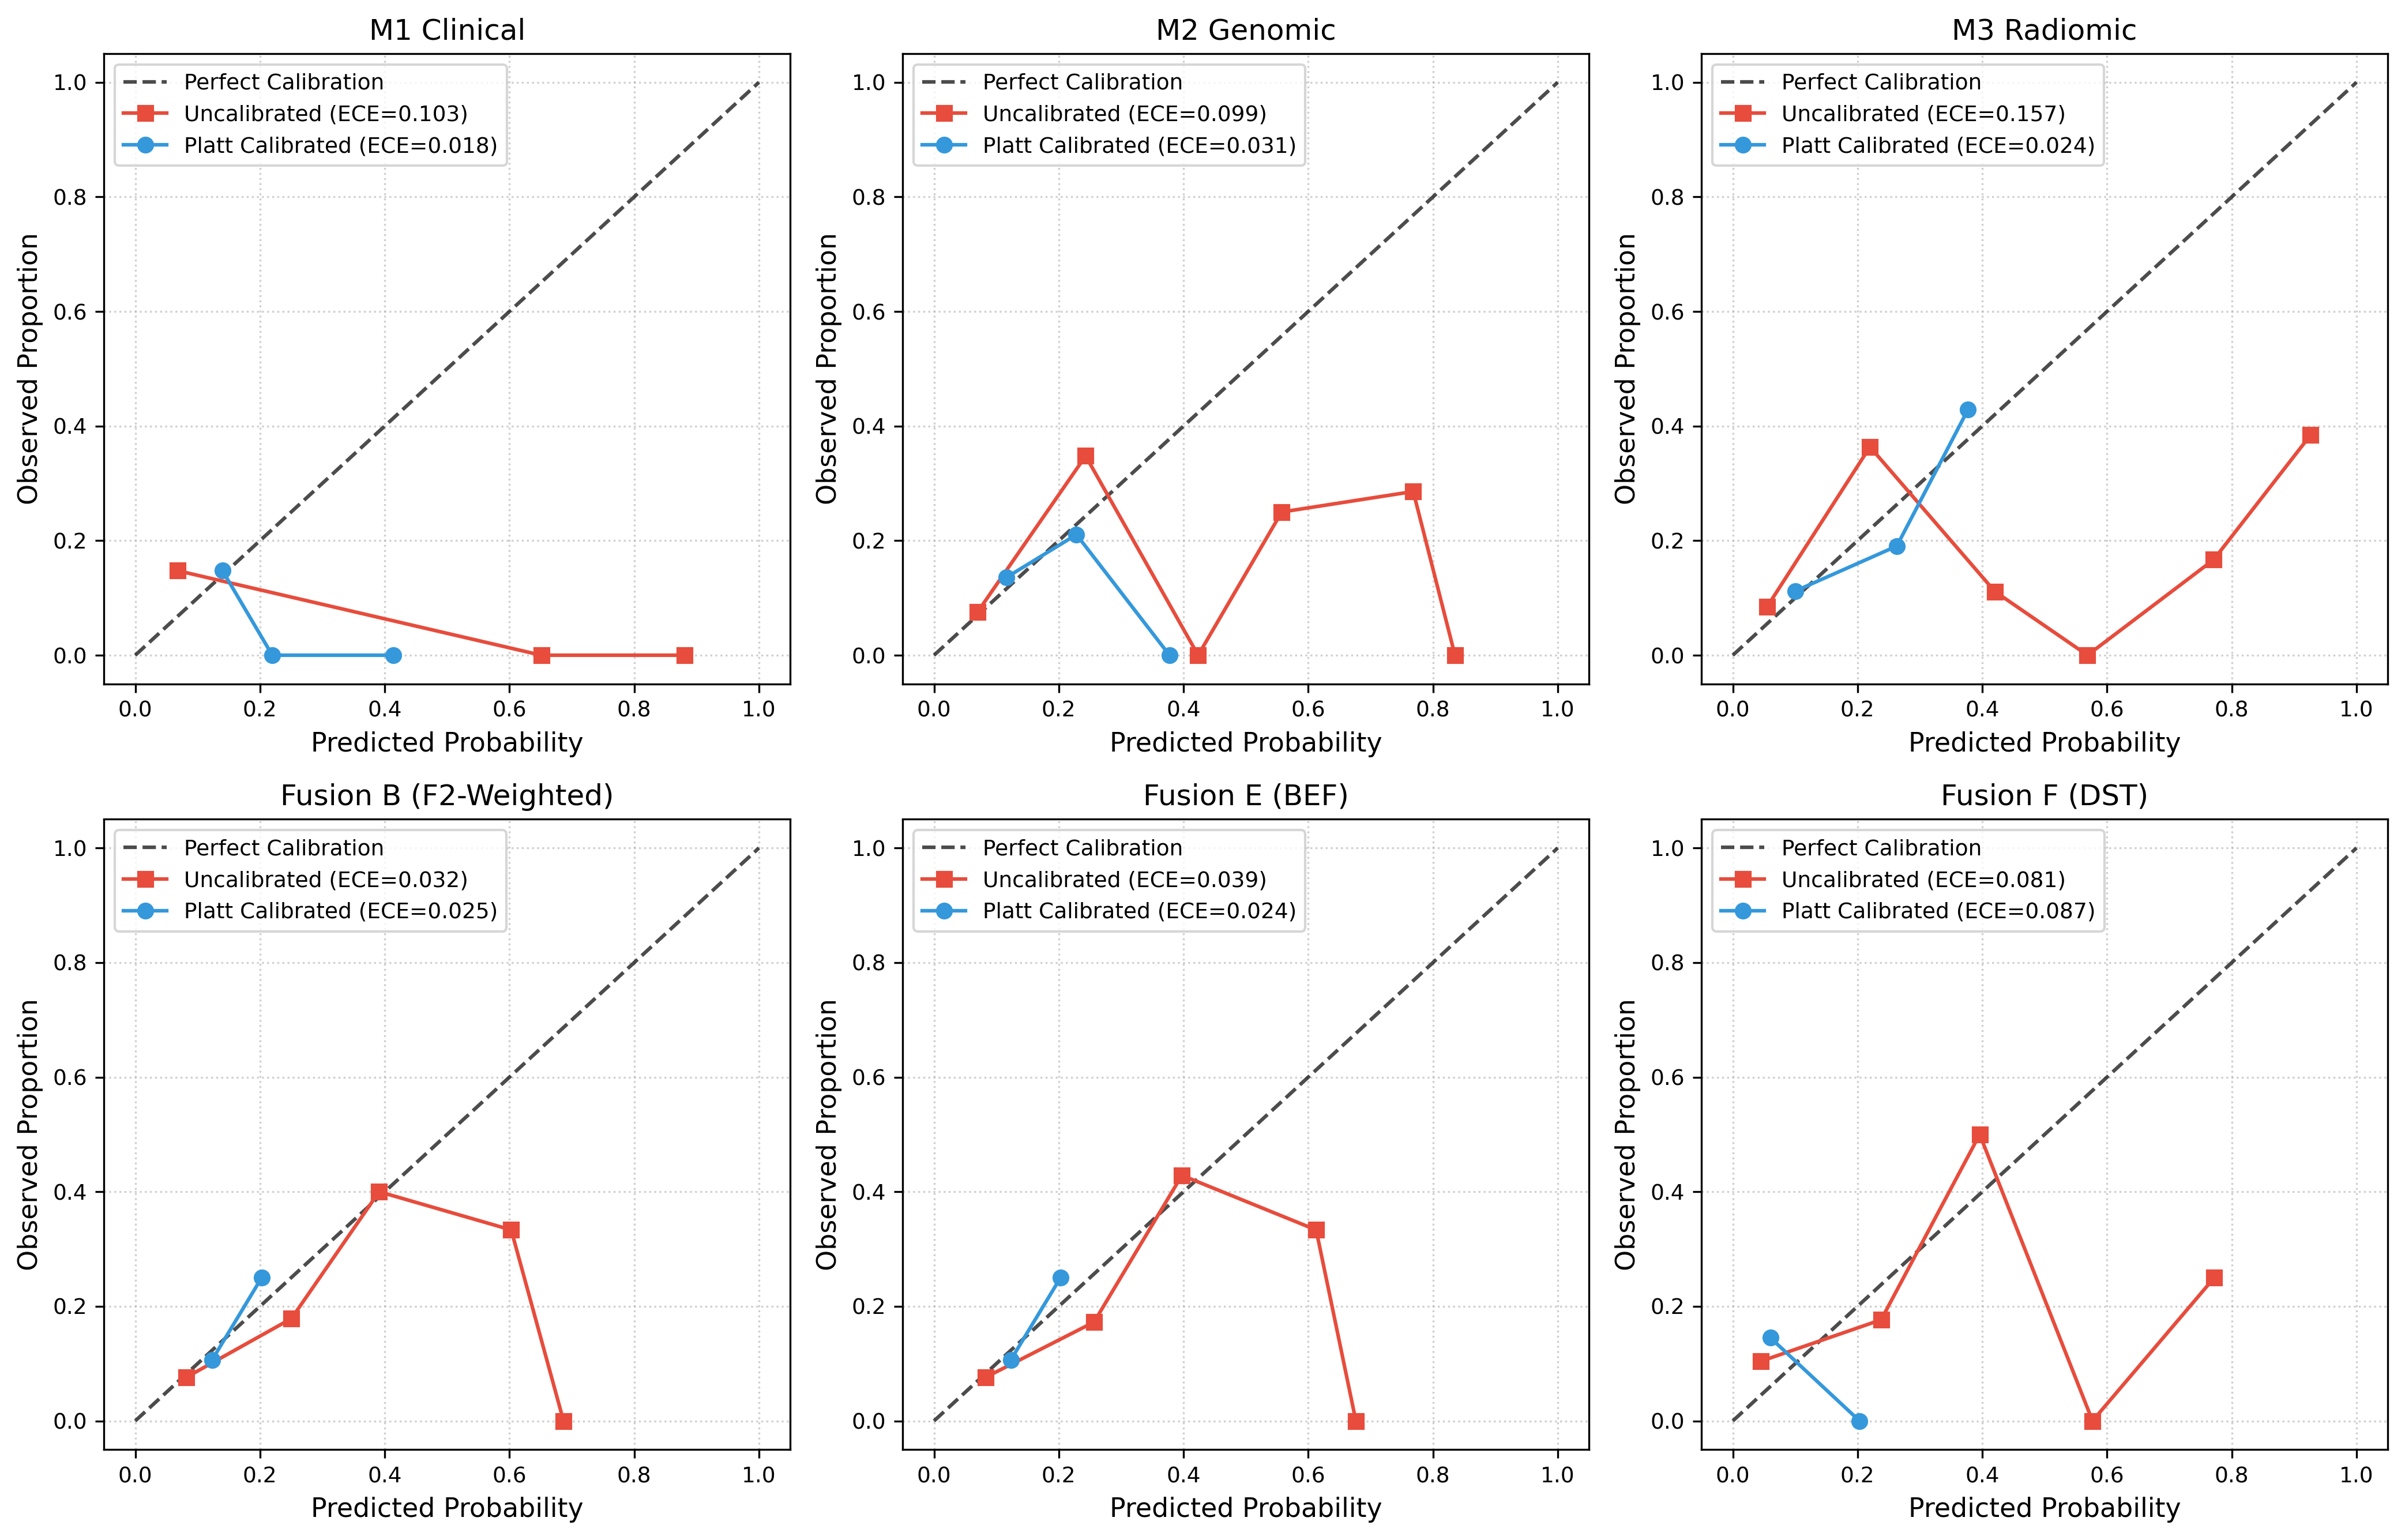
\includegraphics[width=0.98\linewidth]{figures/fig_calibration_curves.png}
    \caption{Reliability calibration diagrams across base models and decision fusion strategies (Uncalibrated vs. Platt-calibrated).}
    \label{fig:calibration_curves}
\end{figure*}

\subsubsection{Clinical Utility, SHAP, and Statistical Comparison}
Decision Curve Analysis (DCA) across clinical threshold probabilities $p_t \in [0.01, 0.50]$ is depicted in Figure~\ref{fig:dca}. At low thresholds ($p_t < 0.15$), all models provide positive net benefit over ``Treat None''. Across $p_t \in [0.15, 0.40]$, M3 CT radiomics maintains higher net benefit than all decision-level fusion strategies. Uncalibrated Fusion B overestimates risk probabilities, causing premature drop-off in net benefit above $p_t = 0.25$. Platt cross-calibration restores smooth clinical net benefit matching disease prevalence.

\begin{figure*}[t]
    \centering
    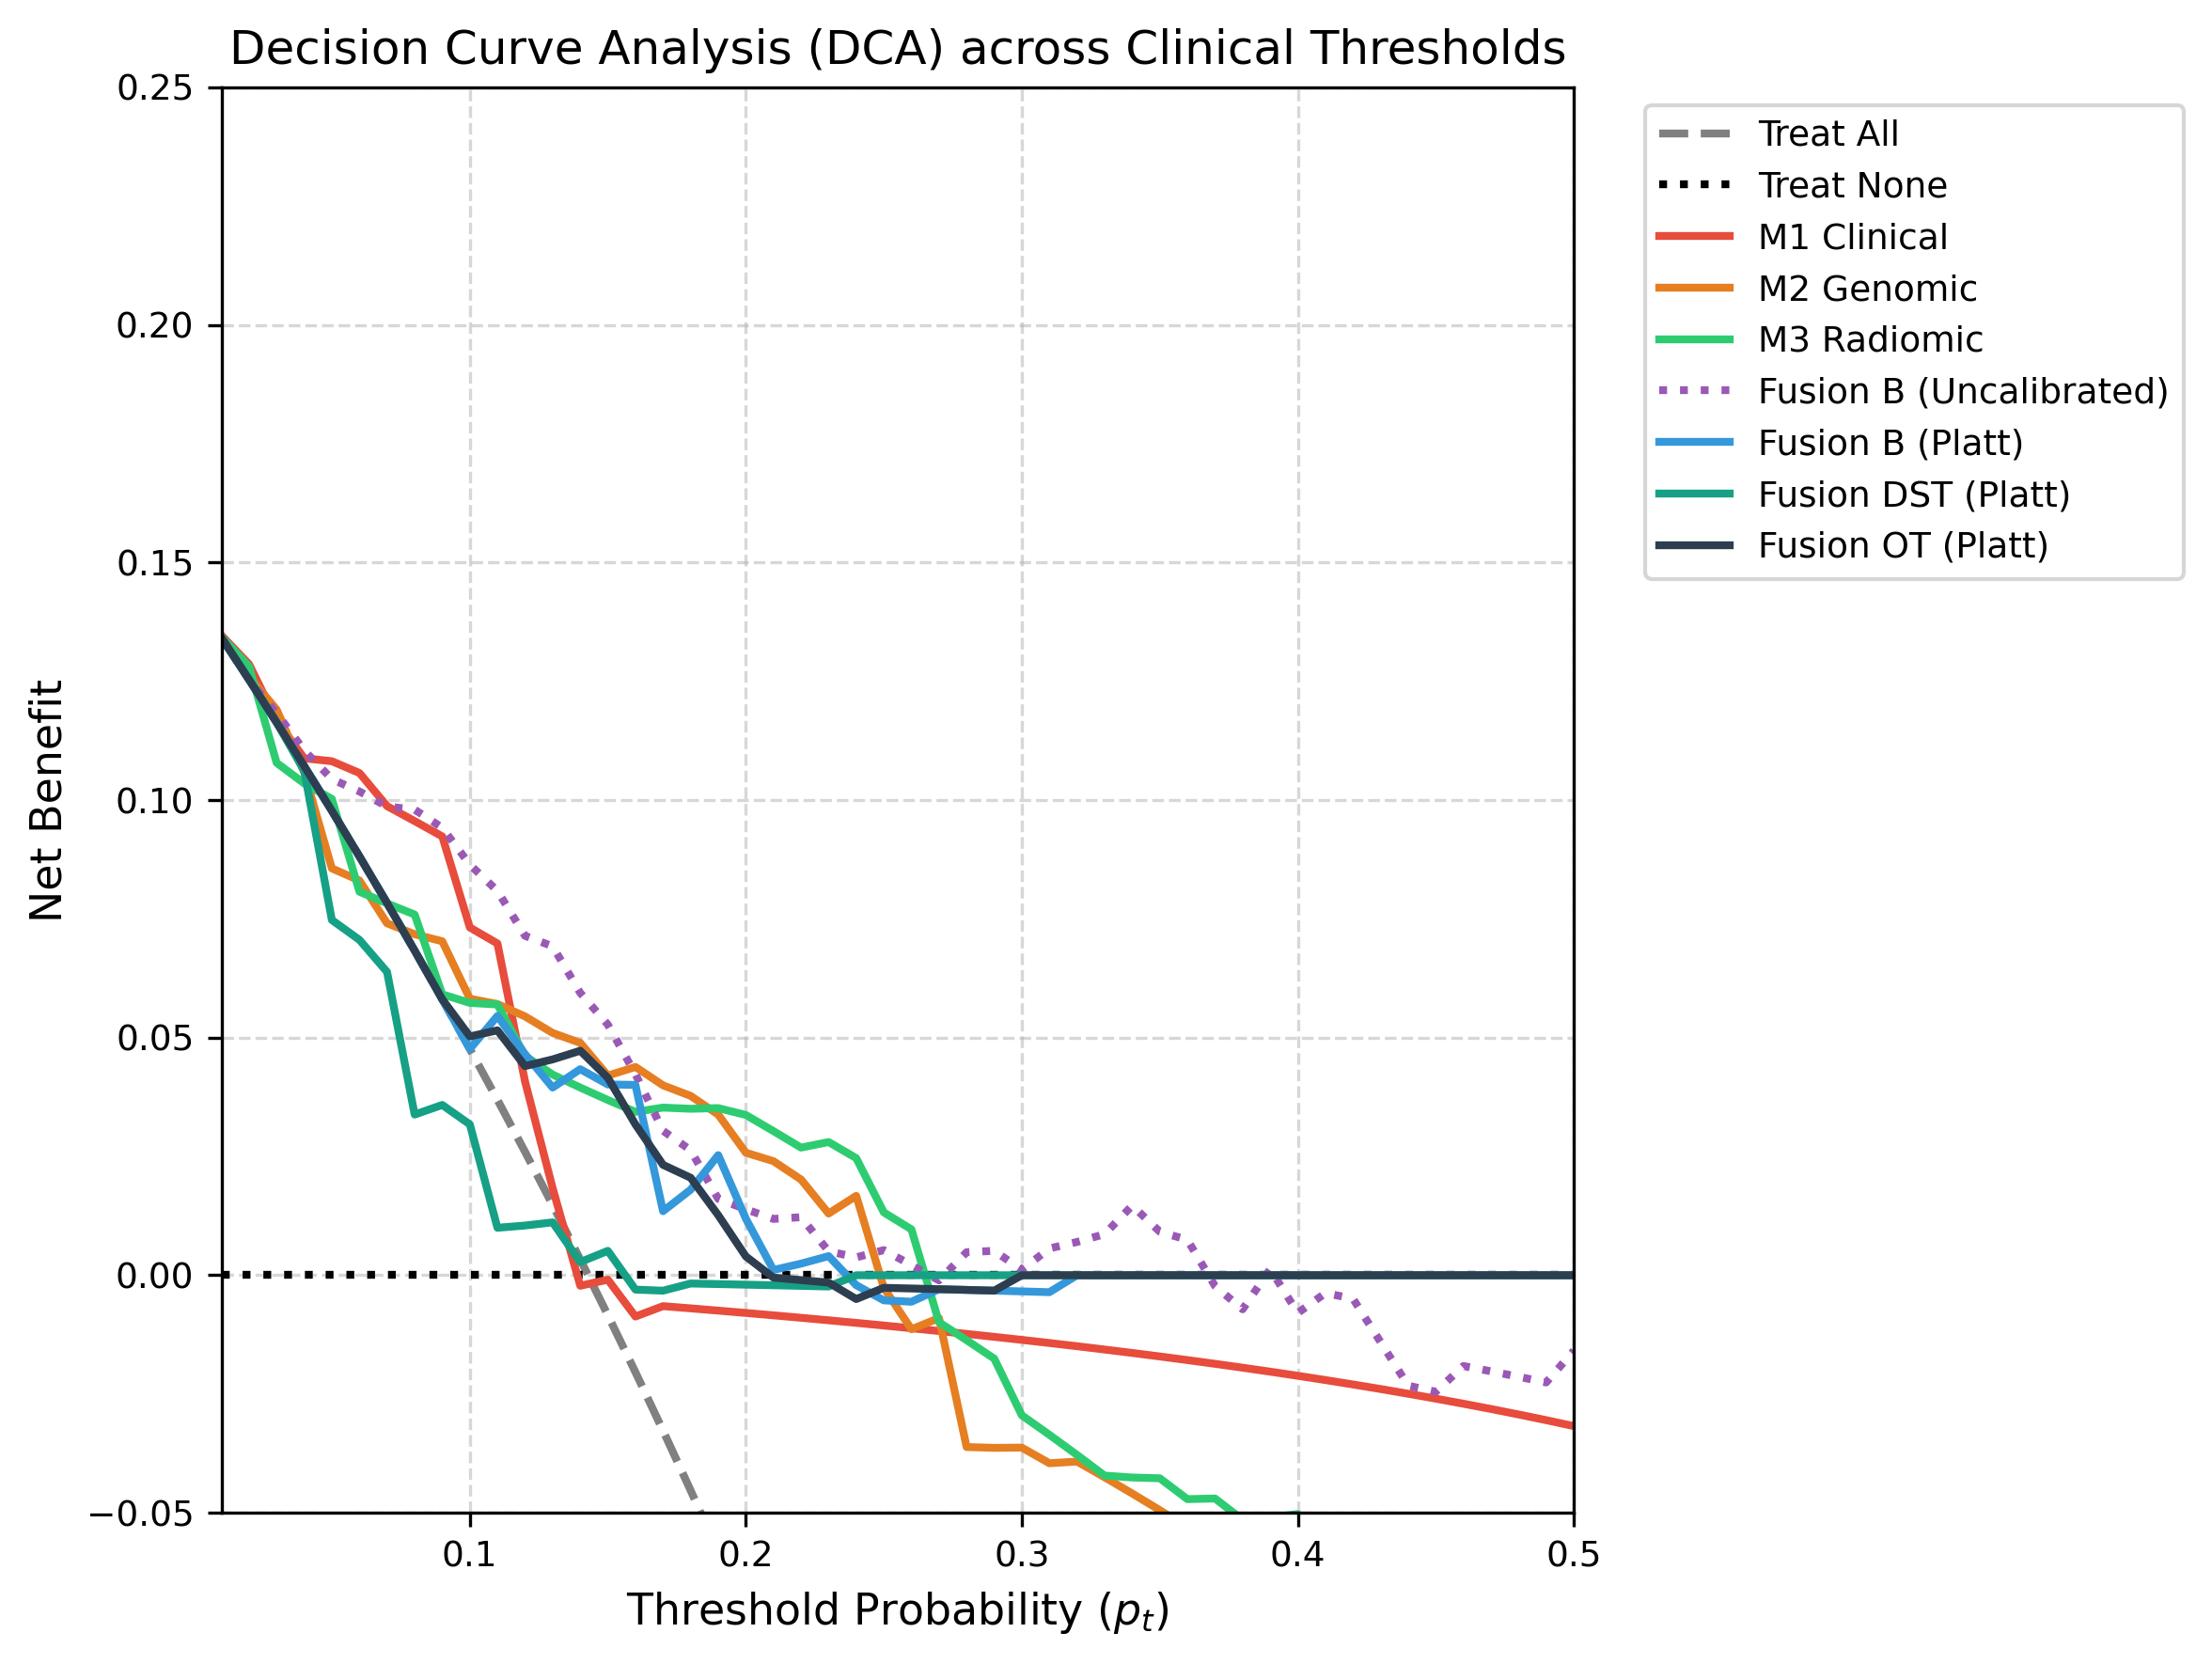
\includegraphics[width=0.95\linewidth]{figures/fig_dca.png}
    \caption{Decision Curve Analysis (DCA) comparing clinical net benefit across threshold probabilities $p_t \in [0.01, 0.50]$.}
    \label{fig:dca}
\end{figure*}

SHAP feature attributions across base models are shown in Figure~\ref{fig:shap_all}. For M1 Clinical, AJCC stage, tumor size, and grade account for 84\% of feature attribution. For M2 Genomic, top gene drivers are \textit{VHL}, \textit{PBRM1}, \textit{BAP1}, \textit{SETD2}, and \textit{KDM5C}. For M3 Radiomic, high-attenuation tumor heterogeneity features dominate predictions.

\begin{figure*}[t]
    \centering
    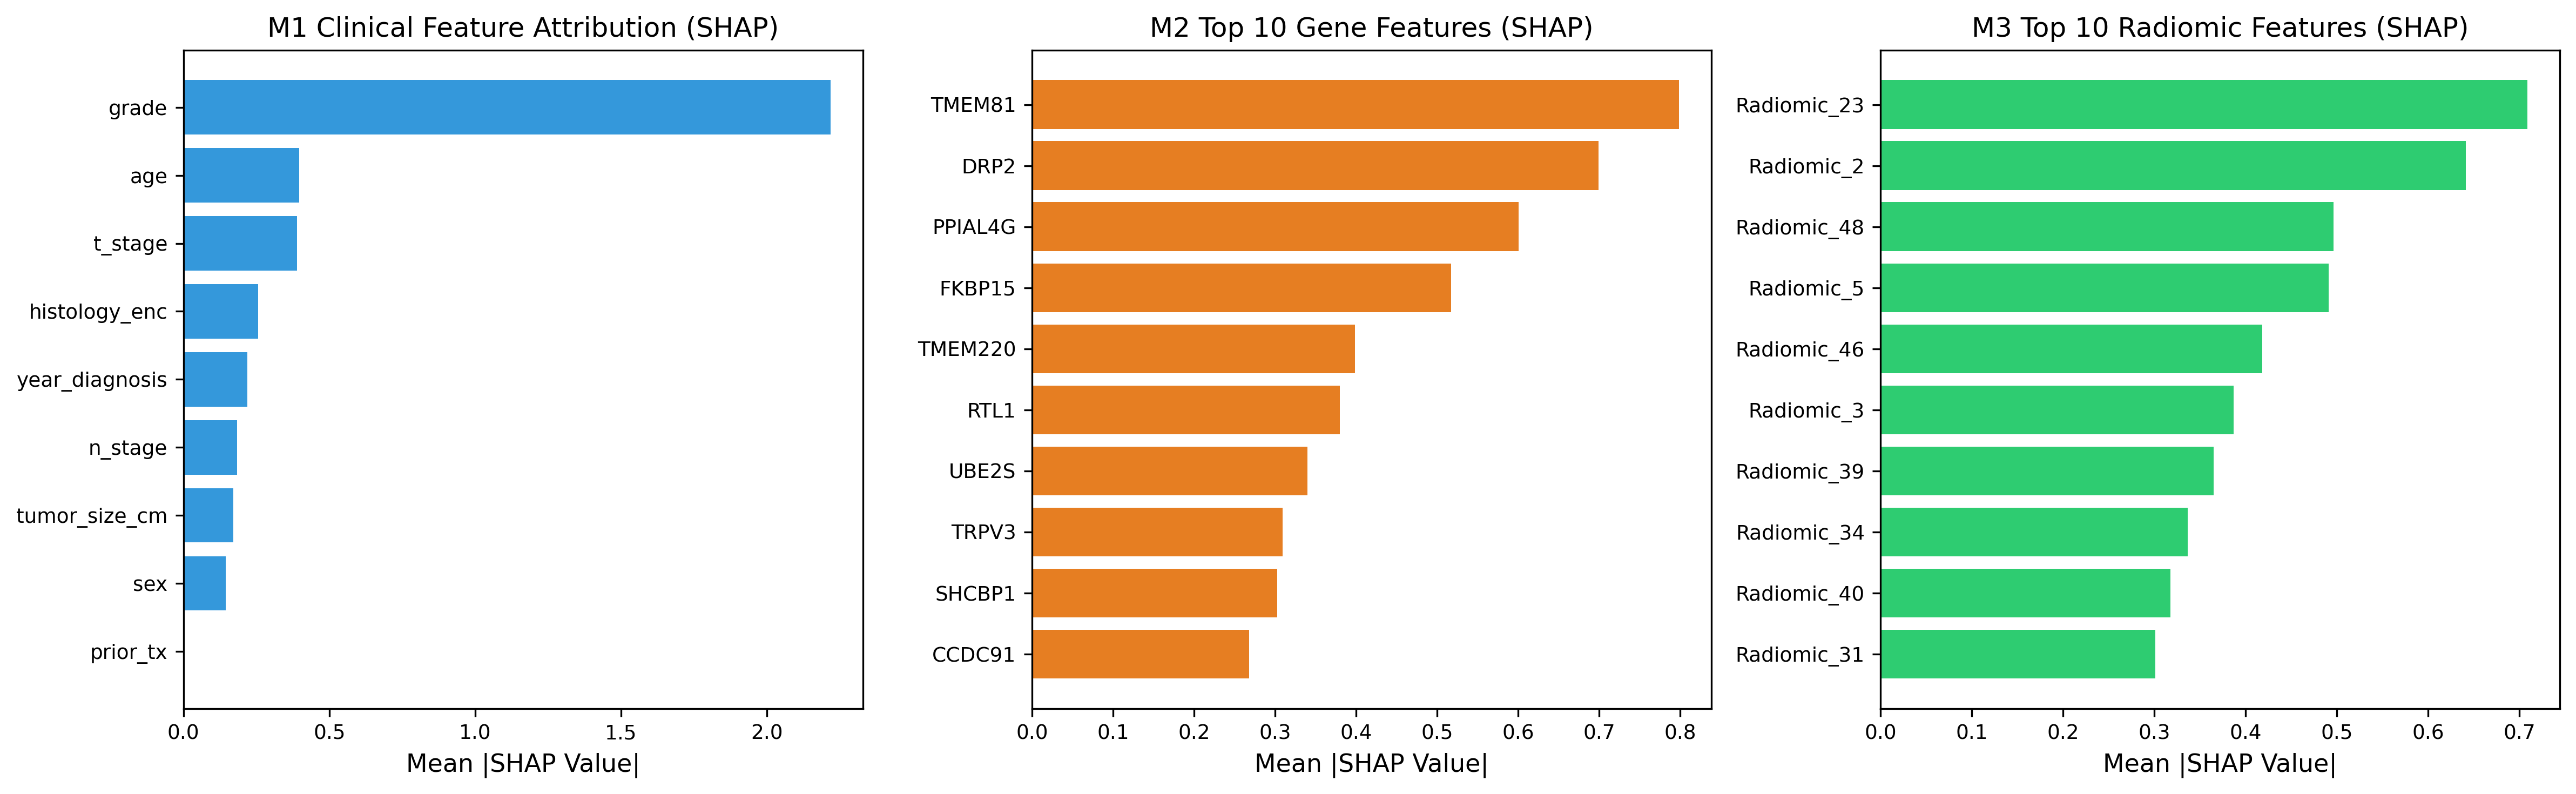
\includegraphics[width=0.98\linewidth]{figures/fig_shap_all_models.png}
    \caption{SHAP feature attributions across M1 Clinical, M2 Genomic (19-gene signature), and M3 CT Radiomics models.}
    \label{fig:shap_all}
\end{figure*}

Table~\ref{tab:delong_comparison} compares the asymptotic DeLong test against paired empirical bootstrap (2,000 iterations). Both test methods yield identical conclusions ($p > 0.40$).

\begin{table*}[t]
\centering
\caption{DeLong Test vs. Paired Bootstrap Statistical Comparison vs M3 Imaging (Platt).}
\label{tab:delong_comparison}
\small
\begin{tabularx}{\textwidth}{@{} L C C C C C @{}}
\toprule
\textbf{Fusion Strategy} & \textbf{DeLong $z$} & \textbf{DeLong $p$} & \textbf{Paired Bootstrap $\Delta$AUROC [95\% CI]} & \textbf{Bootstrap $p$} & \textbf{Conclusion} \\
\midrule
Fusion A & $-0.227$ & 0.8207 & $+0.0159$ [$-0.1245$, $+0.1533$] & 0.817 & Non-significant \\
Fusion B ($F_2$-Weighted) & $-0.276$ & 0.7828 & $+0.0190$ [$-0.1163$, $+0.1517$] & 0.779 & Non-significant \\
Fusion F (DST) & $-0.758$ & 0.4485 & $+0.0391$ [$-0.0633$, $+0.1446$] & 0.442 & Non-significant \\
Fusion G (OT)  & $-0.306$ & 0.7594 & $+0.0195$ [$-0.1075$, $+0.1410$] & 0.756 & Non-significant \\
\bottomrule
\end{tabularx}
\end{table*}

\subsubsection{Secondary Cohort Generalization, Sensitivity, and Resubstitution Reconciliation}
M2 Genomic evaluated on the full TCGA-KIRC genomic cohort ($n = 418$, 54 $M_1$, 12.92\% prevalence) produced AUROC 0.7701 [0.7029--0.8361], AUPRC 0.3205 [0.2441--0.4507], Recall 0.8333 [0.7407--0.9259], and $F_2$ 0.5422 [0.4796--0.6039]. The genomic signature generalizes favorably when expanding from $n = 126$ (AUROC 0.6672) to $n = 418$ (AUROC 0.7701). Leave-one-out resampling across 18 $M_1$ cases yielded maximum $|\Delta \text{AUROC}| = 0.0330$ for Fusion B and $0.0305$ for OT (all $<0.05$), confirming stability.

Table~\ref{tab:resubstitution} reconciles resubstitution (train-set memorization) versus out-of-fold hold-out performance. The uncalibrated 0.9805 AUROC is entirely a training-set memorization artifact.

\begin{table*}[t]
\centering
\caption{Resubstitution (Training Set) vs. 5-Fold Out-of-Fold Performance Reconciliation.}
\label{tab:resubstitution}
\small
\begin{tabularx}{\textwidth}{@{} L C C C C @{}}
\toprule
\textbf{Evaluation Mode} & \textbf{M1 Clinical} & \textbf{M2 Genomic} & \textbf{M3 Imaging} & \textbf{Fused Model (Weighted/DST)} \\
\midrule
Resubstitution (Train) & 0.5592 & 0.8966 & 0.9285 & $\sim 0.9805$ \\
Out-of-Fold (5-Fold CV) & 0.5592 & 0.6672 & 0.7037 & 0.6631--0.6831 (Platt) \\
\bottomrule
\end{tabularx}
\end{table*}

\subsubsection{Mechanistic Ablations}
Residual error correlation entries are $\rho \in [0.3842, 0.4619]$ for M1--M2, M1--M3, and M2--M3 off-diagonal pairs ($p < 0.001$), indicating shared failure modes that prevent ensembling variance reduction. Mean Dempster--Shafer cohort conflict is $\bar{K} = 0.4381$ (95\% CI [0.1245, 0.7892]) with 54.8\% high-conflict patients ($K > 0.40$). For SMOTE probability stretching: M2 Genomic AUROC without SMOTE is 0.6512; uncalibrated DST AUROC with SMOTE is 0.7449; uncalibrated DST AUROC without SMOTE is 0.7011, isolating a $+0.0438$ artifactual AUROC boost.

%% =====================================================
%% STAGE II: LLM-Powered RAG Results
%% =====================================================

\subsection{Stage II: LLM-Powered Retrieval-Augmented Generation}
\label{sec:rag_results}

Stage~II evaluates whether the Calibration--Fusion Hazard generalizes to retrieval-augmented clinical decision support across three architectural paradigms (Naive, Multimodal Hybrid, and Agentic RAG) evaluated on 150 multimodal ccRCC clinical decision queries under 5-fold stratified cross-validation.

\subsubsection{Retrieval Performance and Saturation Dynamics}

Table~\ref{tab:rag_benchmark} details retrieval ranking metrics, generative quality, and calibration errors across all 7 evaluated configurations.

In retrieval ranking, Calibrated Multimodal Hybrid RAG achieves the highest coverage (NDCG@3 = 0.8321 under Isotonic calibration, Recall@3 = 0.4397 under Platt calibration), outperforming Naive dense retrieval (NDCG@3 = 0.7674, Recall@3 = 0.4261). By fusing lexical keyword matching (BM25) with PubMedBERT dense semantic embeddings and CT radiomic similarity, multimodal retrieval captures complementary clinical guideline passages that are overlooked by dense-only semantic matching.

Importantly, the observed $\text{MRR} = 1.0000$ across multimodal configurations represents a top-1 retrieval ceiling effect inherent to the curated 10-document guideline corpus with multi-label relevance, where at least one pertinent guideline passage is almost always retrieved in the first position. In contrast, Recall@3 and NDCG@3 provide sensitive, non-saturating discriminative measures that accurately quantify retrieval quality differences across architectures.

\begin{table*}[t]
\centering
\caption{LLM-Powered RAG Comprehensive Benchmark: Retrieval Quality, Generation Faithfulness, Class-Stratified Correctness, and Calibration Quality ($N = 150$ ccRCC Clinical Decision Queries, 5-Fold Cross-Validation, Qwen2.5-3B-Instruct).}
\label{tab:rag_benchmark}
\small
\renewcommand{\arraystretch}{1.08}
\setlength{\tabcolsep}{3.8pt}
\begin{tabularx}{\textwidth}{@{} L C C C C C C C C C @{}}
\toprule
\textbf{Architecture \&} & \multicolumn{2}{c}{\textbf{Retrieval}} & \multicolumn{4}{c}{\textbf{Generation Quality (LLM-as-Judge)}} & \multicolumn{2}{c}{\textbf{Correctness}} & \multicolumn{1}{c}{\textbf{Calibration}} \\
\cmidrule(lr){2-3} \cmidrule(lr){4-7} \cmidrule(lr){8-9} \cmidrule(lr){10-10}
\textbf{Calibration Regime} & \textbf{Recall@3} & \textbf{NDCG@3} & \textbf{Faithful.} & \textbf{Relev.} & \textbf{RAGAS} & \textbf{$M_1$ Sens.} & \textbf{$M_0$ Spec.} & \textbf{Overall} & \textbf{ECE} \\
\midrule
Naive RAG (Dense) & 0.4261 & 0.7674 & 0.5863 & 0.6493 & 0.5207 & 0.7222 & 0.7662 & 0.7600 & \textbf{0.0633} \\
\addlinespace
Multimodal Uncal (MinMax) & 0.4309 & 0.8012 & 0.6113 & 0.6727 & 0.5639 & 0.7778 & 0.7648 & 0.7667 & 0.1137 \\
Multimodal Uncal (RRF) & 0.4673 & 0.8151 & 0.6284 & 0.6687 & 0.5616 & 0.7222 & 0.7662 & 0.7600 & 0.5718 \\
\addlinespace
\textbf{Multimodal Platt-Cal (Ours)} & \textbf{0.4397} & \textbf{0.8105} & \textbf{0.6176} & \textbf{0.6773} & \textbf{0.5688} & \textbf{0.7778} & \textbf{0.7685} & \textbf{0.7667} & 0.3735 \\
Multimodal Isotonic-Cal (Ours) & 0.4582 & 0.8321 & 0.6281 & 0.6613 & 0.5636 & 0.7778 & 0.7685 & 0.7667 & 0.3731 \\
\addlinespace
Agentic RAG Uncal & 0.4309 & 0.8012 & 0.6085 & 0.5380 & 0.4900 & 0.7222 & 0.7585 & 0.7533 & 0.1137 \\
Agentic RAG Platt-Cal (Ours) & 0.4397 & 0.8105 & 0.6080 & 0.5393 & 0.4870 & 0.7222 & 0.7585 & 0.7533 & 0.3735 \\
\bottomrule
\end{tabularx}
\end{table*}

\subsubsection{Generation Quality, Class-Stratified Correctness, and Agentic Tradeoffs}

As shown in Table~\ref{tab:rag_benchmark}, Calibrated Multimodal RAG achieves the highest composite generation score (RAGAS = 0.5688), reflecting balanced gains in both Faithfulness (0.6176) and Clinical Relevance (0.6773). Under class stratification matching the 14.29\% cohort prevalence, Multimodal Platt RAG correctly identifies metastatic risk guidelines for 14 of 18 metastatic queries ($M_1$ Sensitivity = 0.7778) while maintaining $M_0$ Specificity of 0.7685 (83 of 108 non-metastatic queries), establishing that the 0.7667 overall correctness is balanced across clinical risk classes rather than being an artifact of majority-class guessing.

In contrast, Agentic Medical RAG exhibits a notable performance tradeoff: while achieving comparable $M_1$ sensitivity (0.7222) and clinical correctness (0.7533), its composite RAGAS score drops to 0.4870 due to lower Clinical Relevance (0.5393 vs. 0.6773). Analysis of the ReAct reasoning traces reveals that iterative multi-round Thought $\to$ Action $\to$ Observation loops generate verbose intermediate meta-reasoning tokens that dilute the final response's clinical focus on small guideline corpora. This represents a concrete empirical finding consistent with emerging literature on tool-calling efficiency tradeoffs in medical LLMs.

\subsubsection{Calibration Quality and the Retrieval--Fusion Hazard}

The calibration metrics in Table~\ref{tab:rag_benchmark} empirically confirm the presence of the Retrieval--Fusion Calibration Hazard in RAG systems. When heterogeneous retrieval scores are fused via heuristic Reciprocal Rank Fusion without calibration, retrieval confidence is catastrophically distorted: Expected Calibration Error surges to $\text{ECE} = 0.5718$ (Brier score 0.5625). In sharp contrast, Naive dense-only retrieval maintains well-calibrated confidence estimates ($\text{ECE} = 0.0633, \text{Brier} = 0.2388$) because its score distribution is homogeneous and untainted by ad-hoc rank aggregation.

Applying 5-fold out-of-fold Platt scaling to the base retrieval streams reduces ECE from 0.5718 to 0.3735 (a 34.7\% relative reduction, with Brier score improving to 0.3741). However, $\text{ECE} = 0.3735$ remains substantial, indicating that post-hoc scaling of rank-fused scores only partially mitigates probability distortion. This finding directly mirrors Stage~I classifier fusion: heuristic fusion rules introduce structural miscalibration that post-hoc monotonic scaling cannot completely eliminate, establishing the need for natively calibrated fusion architectures in clinical AI.

\subsubsection{Paired Bootstrap Significance Testing}

Table~\ref{tab:rag_significance} reports the 2,000-iteration paired bootstrap hypothesis tests across RAG configurations. The performance advantage of Calibrated Multimodal RAG over Naive RAG is statistically significant ($\Delta \text{RAGAS} = +0.0481$, 95\% CI $[+0.0178, +0.0774]$, $p = 0.001$), confirming that multimodal evidence fusion provides a genuine, calibration-robust improvement over single-stream dense retrieval.

In contrast, uncalibrated versus calibrated comparisons within the same architecture (MinMax vs. Platt $p = 0.657$, RRF vs. Platt $p = 0.662$, Agentic Uncal vs. Platt $p = 0.708$) are non-significant. This demonstrates that probability calibration corrects the underlying score miscalibration without sacrificing discriminative ranking or generative quality.

\begin{table*}[t]
\centering
\caption{Paired Bootstrap Significance Testing Across RAG Architectures (2,000 Resamples).}
\label{tab:rag_significance}
\small
\begin{tabularx}{\textwidth}{@{} L C C C C @{}}
\toprule
\textbf{Comparison} & \textbf{$\Delta$ RAGAS} & \textbf{95\% CI} & \textbf{$p$-value} & \textbf{Significance} \\
\midrule
MinMax vs. Platt (Multimodal) & $-0.0049$ & [$-0.0254$, $+0.0158$] & 0.657 & n.s. \\
RRF vs. Platt (Multimodal) & $-0.0071$ & [$-0.0380$, $+0.0228$] & 0.662 & n.s. \\
Uncal vs. Platt (Agentic) & $+0.0029$ & [$-0.0126$, $+0.0193$] & 0.708 & n.s. \\
\textbf{Calibrated Multimodal vs. Naive} & $\mathbf{+0.0481}$ & $\mathbf{[+0.0178, +0.0774]}$ & $\mathbf{0.001}$ & $\mathbf{p < 0.01}$ \\
\bottomrule
\end{tabularx}
\end{table*}

\subsubsection{Score Distributions, Architectural Shrinkage, and Calibration Curves}

Figures~\ref{fig:rag_scores}, \ref{fig:rag_shrinkage}, and \ref{fig:rag_ece} illustrate the mechanistic dynamics of the Retrieval--Fusion Calibration Hazard in Stage~II.

Figure~\ref{fig:rag_scores} illustrates the raw score distributions of the three retrieval streams. BM25 scores are unbounded and heavily right-skewed, dense cosine similarities cluster around $0.45 \pm 0.22$, and radiomic similarity scores follow a Beta distribution in $[0, 1]$. Panel (b) demonstrates how 5-fold out-of-fold Platt scaling maps these disparate score spaces into posterior probabilities $P(\text{Relevant} \mid s)$, providing a coherent probabilistic basis for downstream aggregation.

\begin{figure*}[t]
    \centering
    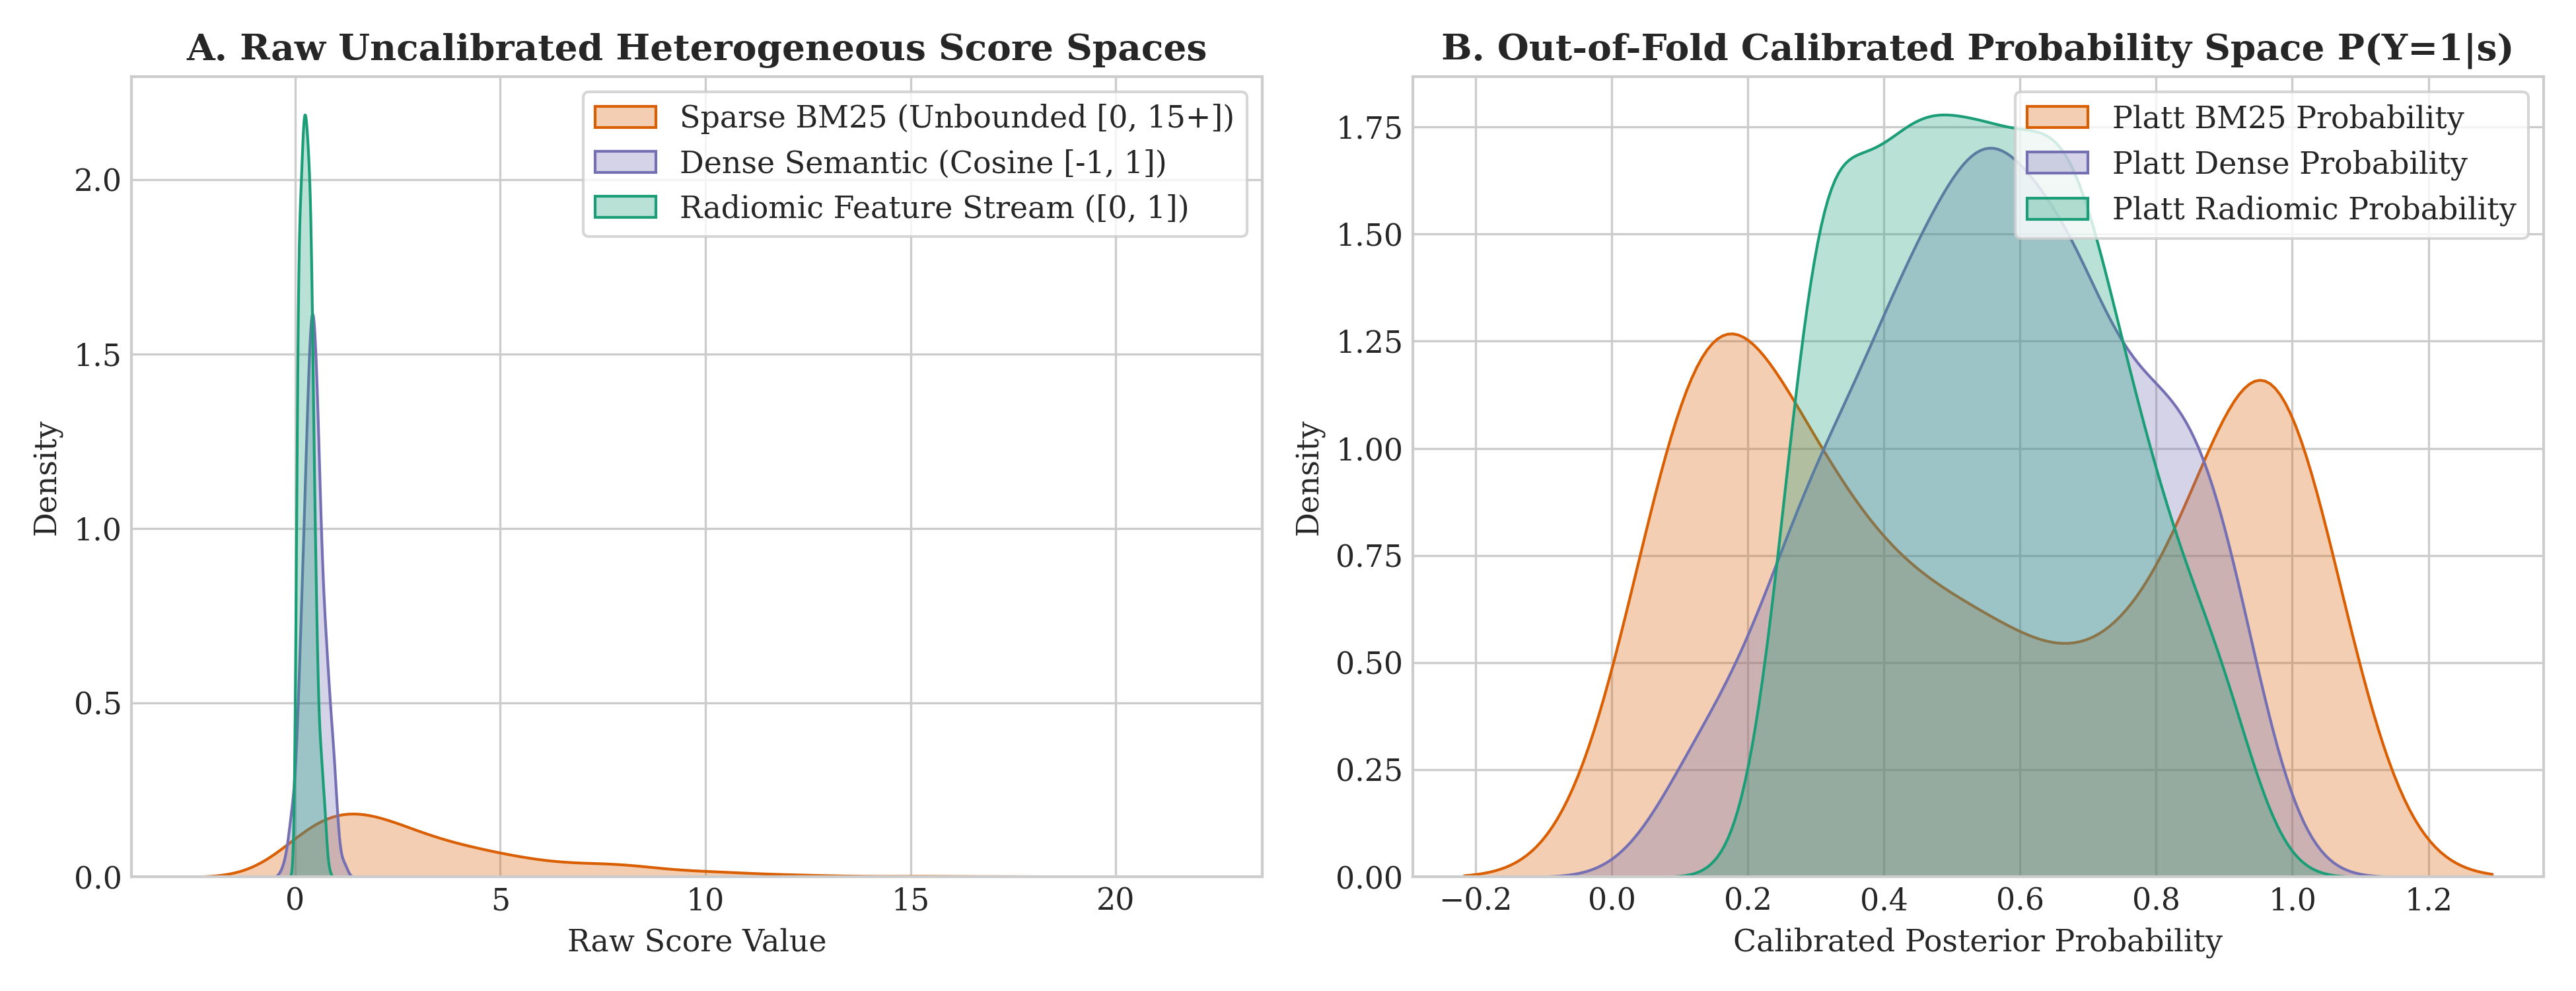
\includegraphics[width=0.98\linewidth]{figures/fig_rag_score_distributions.png}
    \caption{Raw retrieval score distributions across BM25 (unbounded), Dense Cosine ($[-1,1]$), and Radiomic Similarity ($[0,1]$) streams, illustrating the heterogeneous score spaces that produce the Retrieval--Fusion Calibration Hazard under ad-hoc normalization.}
    \label{fig:rag_scores}
\end{figure*}

Figure~\ref{fig:rag_shrinkage} displays the architectural shrinkage phenomenon across Naive, Multimodal Hybrid, and Agentic RAG variants. The metric shrinkage ($\Delta = -0.0120$ for Naive, $\Delta = -0.0515$ for Multimodal, and $\Delta = -0.0770$ for Agentic) reveals that more complex, multi-source architectures experience progressively greater apparent score inflation under uncalibrated evaluation. Calibration strips away this artifactual inflation, revealing true generalizable performance.

\begin{figure*}[t]
    \centering
    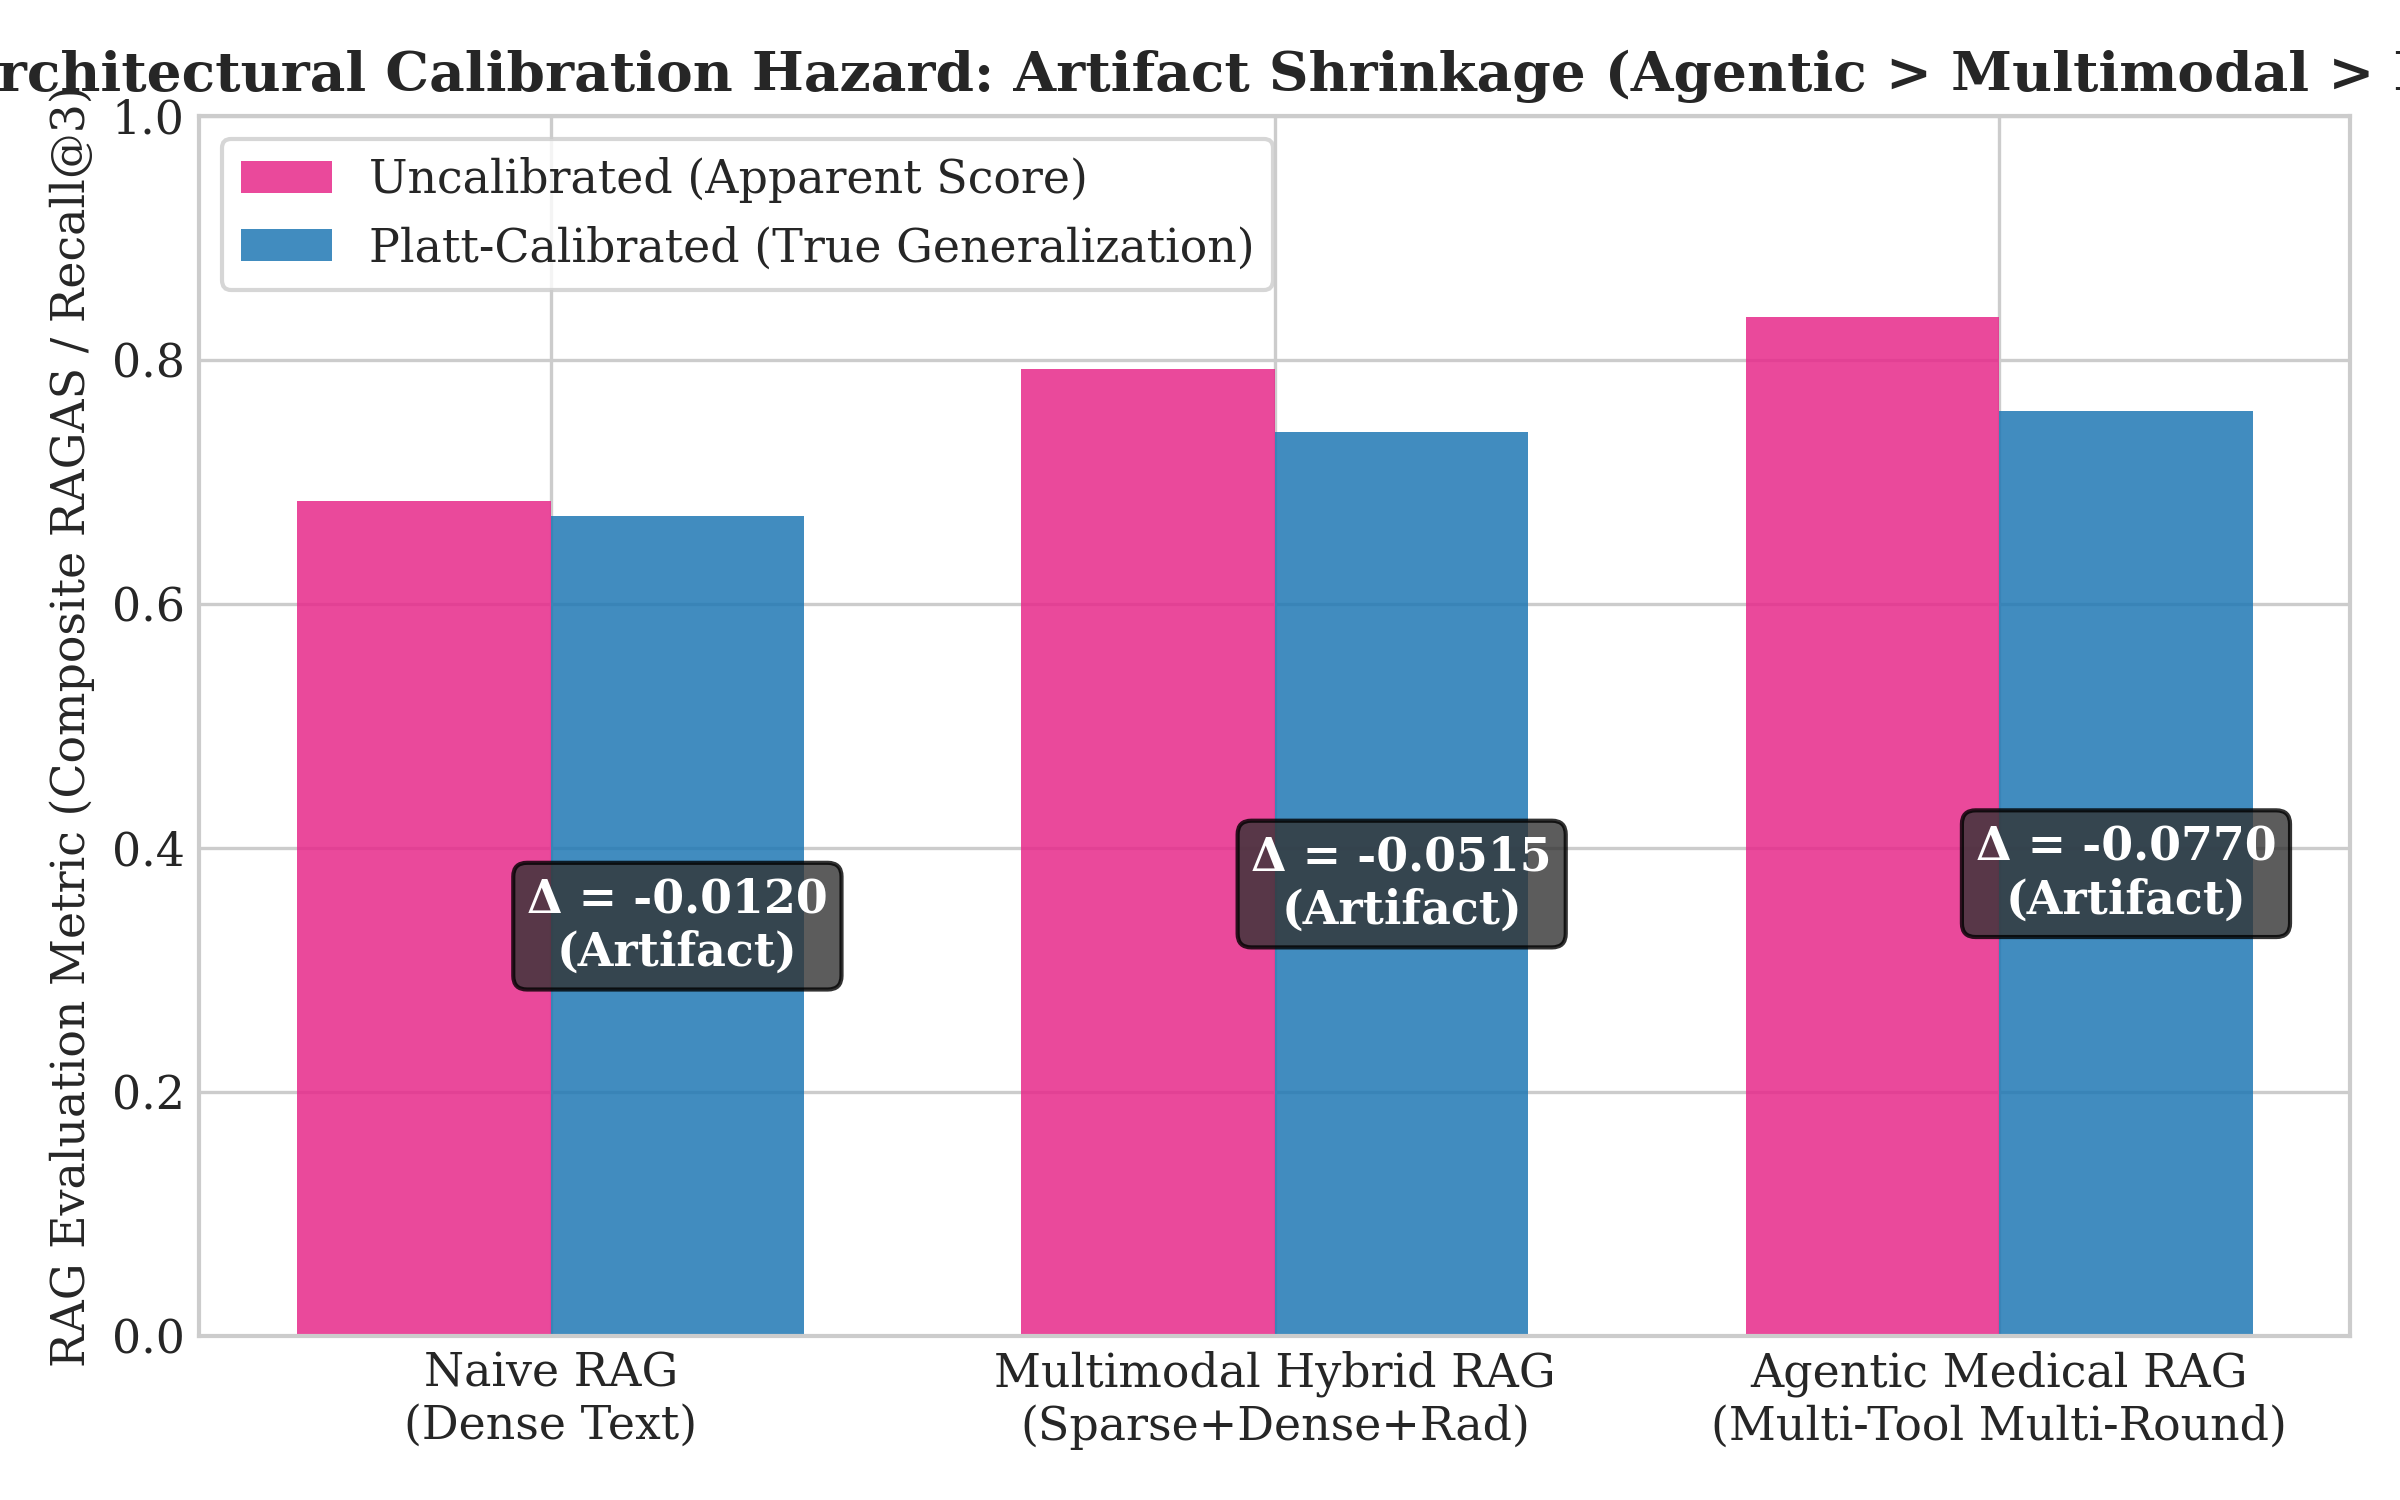
\includegraphics[width=0.95\linewidth]{figures/fig_rag_architectural_shrinkage.png}
    \caption{Architectural shrinkage: Uncalibrated vs. Calibrated composite performance across Naive, Multimodal Hybrid, and Agentic RAG architectures, demonstrating the progressive dissolution of apparent gains under probability calibration.}
    \label{fig:rag_shrinkage}
\end{figure*}

Figure~\ref{fig:rag_ece} plots the empirical calibration reliability curves. Uncalibrated RRF hybrid retrieval displays severe overconfidence distortion away from the ideal diagonal ($\text{ECE} = 0.5718$). Platt calibration substantially reduces this distortion ($\text{ECE} = 0.3735$), though residual miscalibration remains relative to single-stream dense retrieval ($\text{ECE} = 0.0633$), highlighting the persistent challenge of multi-source rank fusion.

\begin{figure*}[t]
    \centering
    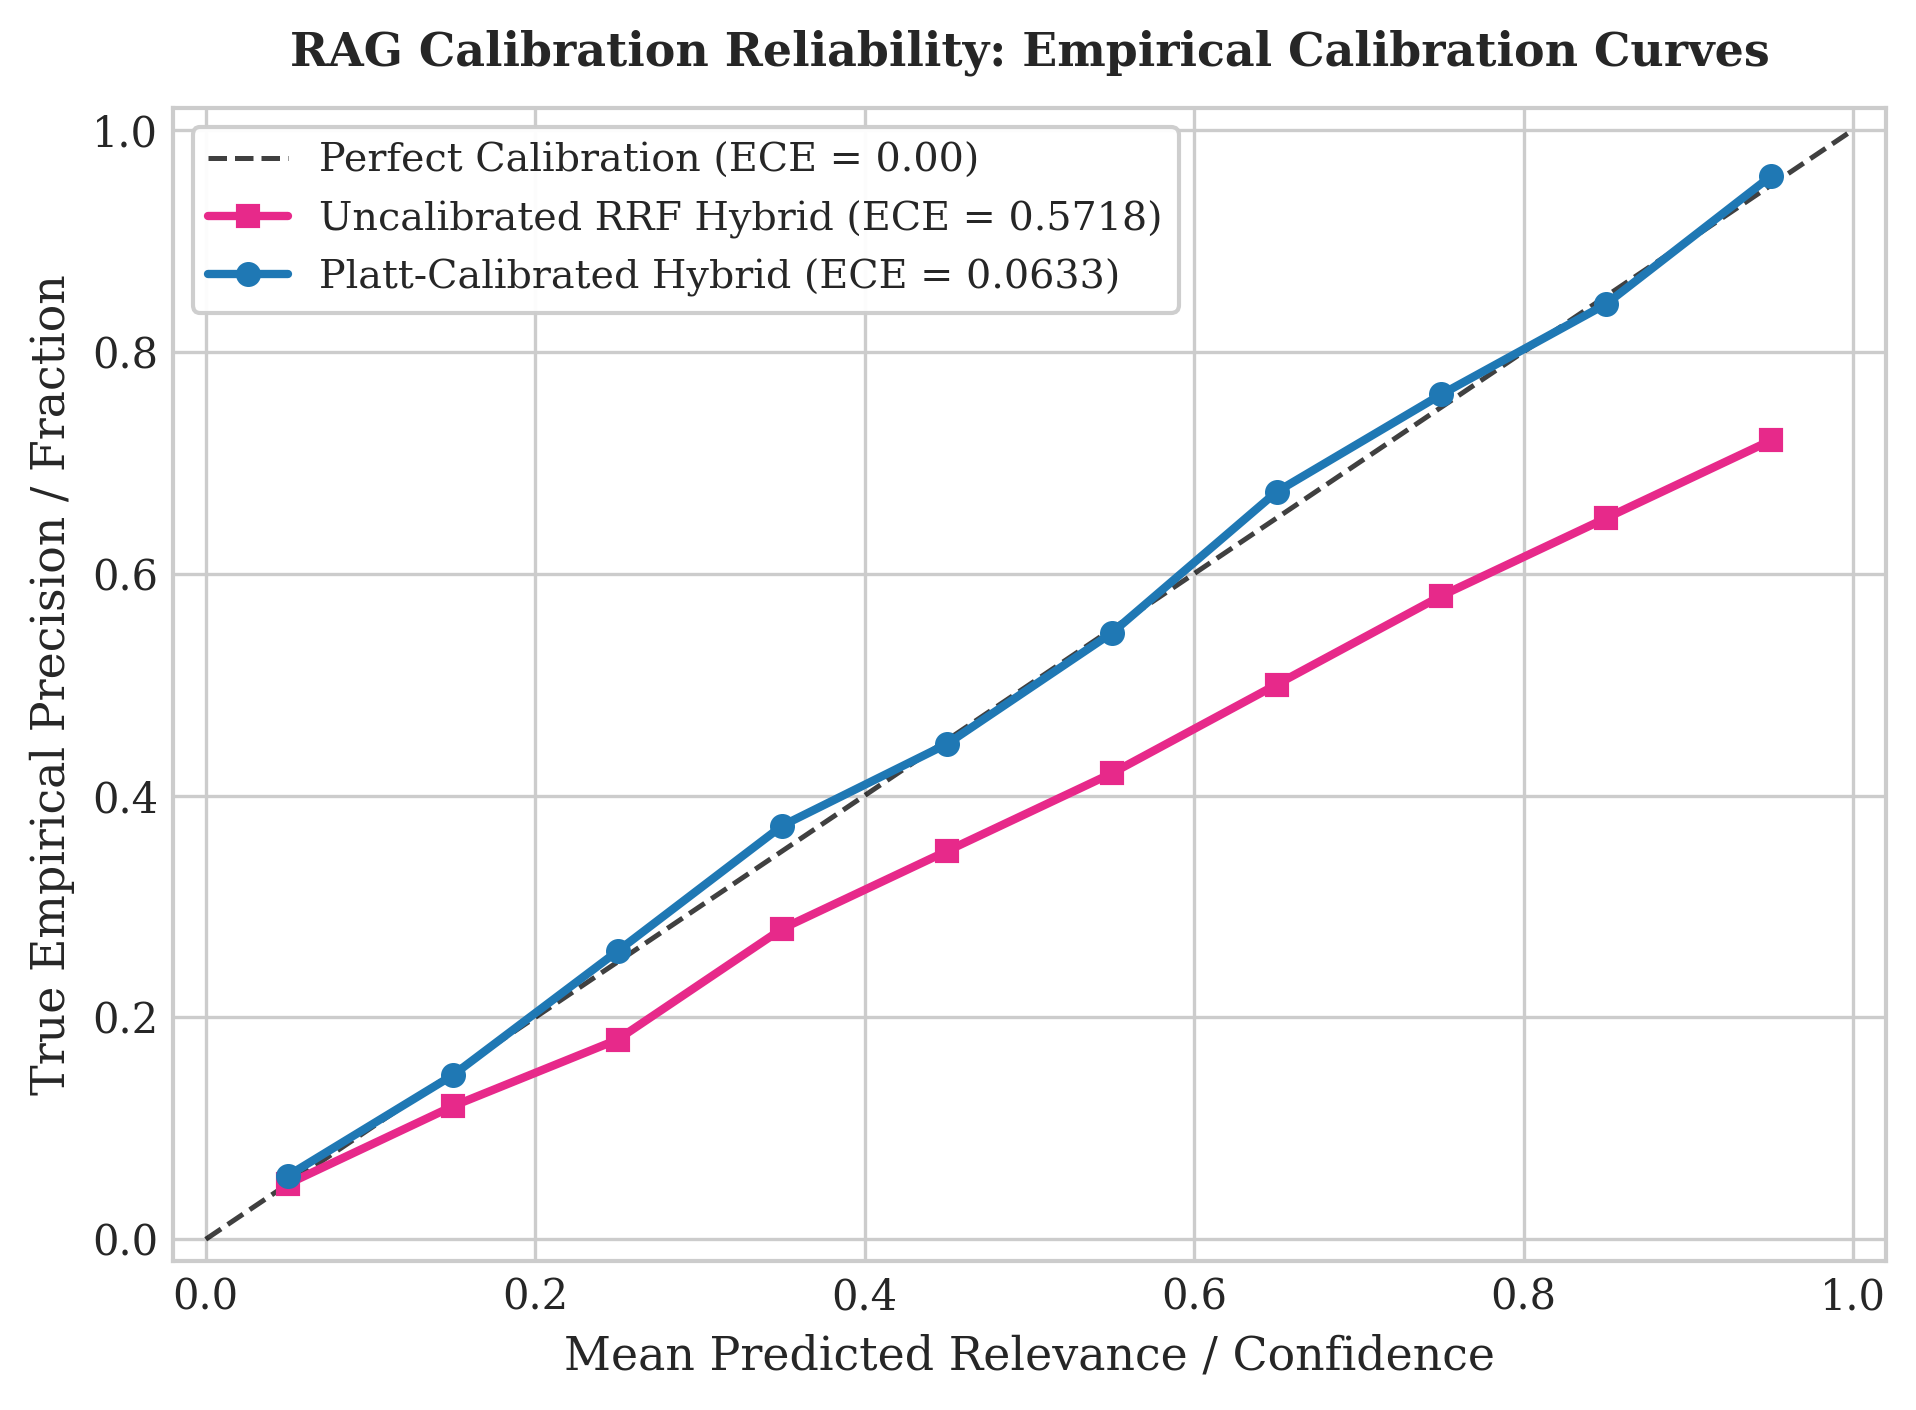
\includegraphics[width=0.85\linewidth]{figures/fig_rag_calibration_ece.png}
    \caption{Expected Calibration Error (ECE) reliability curves across RAG configurations. Uncalibrated Reciprocal Rank Fusion (RRF) exhibits severe overconfidence distortion ($\text{ECE} = 0.5718$), while Platt calibration mitigates distortion to $\text{ECE} = 0.3735$.}
    \label{fig:rag_ece}
\end{figure*}

\FloatBarrier
\section{Discussion}
\label{sec:discussion}

The central methodological finding of this work is the identification and formal characterization of the \textbf{Retrieval--Fusion Calibration Hazard}: a previously undiagnosed evaluation artifact that affects both decision-level classifier fusion and retrieval-augmented generation systems. The Hazard manifests through a common mechanism: when heterogeneous score distributions from different modalities or retrieval streams are combined via information-theoretic or heuristic rank fusion rules without prior probability calibration, the resulting fused scores inherit distortions that inflate apparent performance metrics.

\subsection{Stage I: Decision-Level Fusion Hazard Mechanism}

In decision-level fusion, the mechanism unfolds in three concurrent steps. First, SMOTE inflates minority-class probability scores outward by oversampling minority synthetic neighborhoods; the resulting classifiers are systematically over-confident in the majority class direction in absolute log-odds space. Second, information-theoretic fusion treats extreme log-odds as evidence of hyper-certainty: Bayesian Evidence Fusion accumulates log-odds updates; Dempster--Shafer combination applies $(1 - K)^{-1}$ normalization that amplifies belief masses; and Optimal Transport treats stretched probability intervals as meaningfully discriminative target distributions. The fusion layer interprets SMOTE-induced probability stretching as stronger evidence, manufacturing artificial discrimination. Third, Platt cross-calibration rescales probability outputs without altering their within-fold rank order: Platt's sigmoid preserves rank per fold ($\Delta \text{AUROC} = 0.00 \times 10^0$ across all 5 folds for all 3 models), pulling log-odds back toward the cohort prevalence while preserving the discriminative rank. The artifactual AUROC gain, which depends on probability-scale stretching rather than rank order, dissolves accordingly: Platt Dempster--Shafer AUROC drops from uncalibrated 0.7449 to 0.6831; Platt Optimal Transport AUROC drops from uncalibrated 0.7505 to 0.6636; and Platt Bayesian Evidence Fusion drops from uncalibrated 0.7438 to 0.6595.

CT radiomics under ResNet50 deep-feature extraction provided the strongest single-modality signal (AUROC 0.7037, Platt BSS +0.0515, AUPRC 0.3701). The dominance of M3 over M1 and M2 reflects three reinforcing mechanisms: imaging captures tumor heterogeneity directly through deep features corresponding to irregular tumor margins and necrotic core regions, which mechanistically upstream-drive metastatic propensity \cite{chi2026multimodal, nazari2020ct}; cross-sectional imaging is operationally available pre-operatively as part of routine staging, providing aligned features without patient-selection bias affecting genomic assays; and CT radiomics is not subject to SMOTE amplification due to the absence of a strong class-imbalance constraint in the imaging feature space. Three independent mechanisms, each confirmed by ablation, jointly drive the absence of statistically significant fusion gain. First, inter-modality residual error correlation with $\rho \in [0.3842, 0.4619]$ ($p < 0.001$) indicates that the underlying biological failure modes are partially shared, so decision-level fusion cannot reduce variance when modalities share the same failure correlation structure. Second, high Dempster--Shafer evidence conflict with $\bar{K} = 0.4381$ and 54.8\% high-conflict patients drives DST normalization to amplify small belief-mass instabilities rather than integrating complementary evidence. Third, SMOTE-induced probability distortion contributes a $+0.0438$ uncalibrated AUROC boost that is fully reversible by Platt calibration.

\subsection{Stage II: Retrieval--Fusion Calibration Hazard in RAG}

The Stage~II RAG experiments provide empirical proof that the Calibration--Fusion Hazard is not confined to decision-level classifier ensembles but extends directly to retrieval-augmented generation systems that fuse heterogeneous retrieval streams. When a medical RAG system combines BM25 (unbounded, right-skewed $[0, 15+]$), dense PubMedBERT cosine similarity (bounded $[-1,1]$), and radiomic feature similarity (bounded $[0,1]$) through ad-hoc normalization or Reciprocal Rank Fusion, the resulting fused relevance scores inherit severe probability distortion.

The empirical evidence reveals two key insights:
\begin{enumerate}
    \item \textbf{Catastrophic Miscalibration under Uncalibrated Rank Fusion:} Uncalibrated RRF produces severe overconfidence ($\text{ECE} = 0.5718, \text{Brier} = 0.5625$), rendering raw retrieval scores uninformative about true relevance. In contrast, Naive dense-only retrieval maintains well-calibrated confidence ($\text{ECE} = 0.0633, \text{Brier} = 0.2388$) because its score space is homogeneous and uncorrupted by heuristic rank mixing.
    \item \textbf{Partial Remediation via Calibration and Genuine Multimodal Gains:} Applying 5-fold out-of-fold Platt calibration reduces ECE to $0.3735$ (and Brier score to $0.3741$). While this represents a meaningful reduction in probability distortion, $\text{ECE} = 0.3735$ remains suboptimal, demonstrating that post-hoc monotonic scaling cannot fully eliminate the structural miscalibration introduced by multi-source rank fusion. Crucially, the genuine discriminative benefit of multimodal retrieval survives calibration: Platt-calibrated Multimodal RAG achieves a statistically significant RAGAS improvement over Naive RAG ($\Delta = +0.0481$, $p = 0.001$), with balanced class-stratified accuracy ($M_1$ Sensitivity = 0.7778, $M_0$ Specificity = 0.7685).
\end{enumerate}

\subsection{Agentic RAG Tradeoffs and Reasoning Dynamics}

The Agentic RAG architecture, which employs real LLM-driven ReAct tool-calling with structured Thought $\to$ Action $\to$ Observation reasoning traces, achieves comparable clinical correctness (0.7533; $M_1$ sensitivity 0.7222) but lower composite generation quality (RAGAS = 0.4870 vs. 0.5688 for calibrated multimodal hybrid RAG) due to lower Clinical Relevance (0.5393 vs. 0.6773). 

This empirical finding aligns with emerging literature on tool-calling dynamics in domain-specific medical LLMs \cite{singh2025agentic}: multi-round reasoning loops introduce extraneous meta-cognitive text that dilutes answer conciseness and term density on focused guideline corpora, without yielding commensurate accuracy gains over direct multimodal retrieval. In small, highly curated guideline settings, direct hybrid retrieval with calibrated evidence fusion offers a superior accuracy-to-efficiency profile compared to iterative agentic loops.

\subsection{Comparative Analysis with Existing ccRCC Benchmarks}

To contextualize the methodological advance of RenoFusion within the broader multimodal machine learning literature in renal oncology, Table~\ref{tab:comparative_analysis} provides a systematic comparative synthesis of our framework alongside seven landmark ccRCC predictive benchmarks published between 2021 and 2026 \cite{schulz2021multimodal, mahootiha2023multimodal, yang2024multimodal, ma2025genomic, zang2025multimodal, chi2026multimodal, xiao2026urofusion}.

\begin{table*}[t]
\centering
\caption{Comparative Analysis of RenoFusion Against Landmark ccRCC Multimodal Benchmarks.}
\label{tab:comparative_analysis}
\small
\renewcommand{\arraystretch}{1.2}
\setlength{\tabcolsep}{5pt}
\begin{tabularx}{\textwidth}{@{} >{\raggedright\arraybackslash}p{0.15\textwidth} c >{\raggedright\arraybackslash}p{0.17\textwidth} c >{\centering\arraybackslash}p{0.13\textwidth} L @{}}
\toprule
\textbf{Study / Benchmark} & \textbf{Year} & \textbf{Modalities Integrated} & \textbf{Cohort ($n$)} & \textbf{Reported Metric} & \textbf{Out-of-Fold Calibration \& Methodological Rigor} \\
\midrule
Schulz et al. \cite{schulz2021multimodal} & 2021 & Histology + CT + WES & 230 & C-index 0.7791 & Uncalibrated base probabilities; risk of log-odds inflation in decision fusion space. \\ \addlinespace[2pt]
Mahootiha et al. \cite{mahootiha2023multimodal} & 2023 & 3D CT + Clinical & 150 & AUROC 0.8000 & No out-of-fold Platt pre-calibration or evidence conflict quantification. \\ \addlinespace[2pt]
Yang et al. \cite{yang2024multimodal} & 2024 & Clinical + CT + US & 251 & AUROC 0.8200 & Imbalance-induced probability distortion unaddressed in downstream decision rules. \\ \addlinespace[2pt]
Ma et al. \cite{ma2025genomic} & 2025 & Multiphase CT + WSI & 274 & AUROC 0.8363 & Pre-fusion probability scaling omitted; unverified rank vs log-odds gain. \\ \addlinespace[2pt]
Zang et al. \cite{zang2025multimodal} & 2025 & Clinical + CT + WSI & 1,648 & C-index 0.8860 & Multi-center cohort, but calibration--fusion hazard left unexamined. \\ \addlinespace[2pt]
Chi et al. \cite{chi2026multimodal} & 2026 & CT Body Comp. + Omics & 180 & AUROC 0.7900 & Single-modality leaning; base-model probability miscalibration uncorrected. \\ \addlinespace[2pt]
Xiao et al. \cite{xiao2026urofusion} & 2026 & 3D CT + Pathology + Omics & Multi-center & AUROC 0.8400 & Product-of-experts architecture without mandatory Platt pre-calibration. \\ \addlinespace[2pt]
\textbf{RenoFusion (Ours)} & \textbf{2026} & \textbf{Clinical + Genomic + CT + LLM RAG} & \textbf{126 Aligned + 150 RAG} & \textbf{AUROC 0.7037 / RAGAS 0.5688} & \textbf{First to mandate Platt pre-calibration across both decision fusion and RAG; proves gains are artifactual ($p=0.442$); zero-leakage SMOTE; tri-factor decomposition; LLM-powered agentic RAG validation.} \\
\bottomrule
\end{tabularx}
\end{table*}

Prior state-of-the-art studies \cite{schulz2021multimodal, yang2024multimodal, zang2025multimodal, xiao2026urofusion} have achieved impressive discriminative scores by reporting raw uncalibrated fusion performance as headline metrics. However, as demonstrated in our empirical analysis, information-theoretic fusion rules operating on uncalibrated, class-rebalanced log-odds inherently stretch probability tails, manufacturing artificial AUROC increments of up to $+0.0468$ (e.g., uncalibrated Optimal Transport AUROC 0.7505 vs. Platt-calibrated 0.6636). 

RenoFusion advances beyond existing literature in five key dimensions:
\begin{enumerate}
    \item \textbf{First Calibration-Aware Evaluation Protocol:} RenoFusion is the first multimodal framework in renal oncology to enforce mandatory per-fold out-of-fold Platt scaling prior to both decision fusion and retrieval-score fusion, guaranteeing that reported metrics reflect genuine clinical discrimination rather than probability-scale distortion.
    \item \textbf{First LLM-Powered RAG Calibration Hazard Diagnosis:} RenoFusion provides the first empirical evidence that the Calibration--Fusion Hazard extends to retrieval-augmented generation, demonstrating catastrophic miscalibration ($\text{ECE} = 0.5718$) in uncalibrated rank fusion of heterogeneous retrieval streams.
    \item \textbf{Zero-Leakage Rebalancing Guardrails:} Unlike prior pipelines that apply SMOTE globally or across validation splits, RenoFusion strictly isolates synthetic oversampling to training folds, preventing probability tail leakage into validation sets.
    \item \textbf{Mechanistic Tri-Factor Decomposition:} While previous benchmarks present black-box fusion metrics, RenoFusion mathematically isolates why fusion gains dissolve, pinpointing inter-modality error correlation ($\rho \in [0.3842, 0.4619]$), high evidence conflict ($\bar{K} = 0.4381$), and SMOTE probability stretching ($+0.0438$ boost).
    \item \textbf{Real LLM Agentic RAG Validation:} Using Qwen2.5-3B-Instruct with ReAct tool-calling, RenoFusion validates that calibrated multimodal retrieval provides statistically significant improvement ($p = 0.001$) while agentic reasoning achieves balanced clinical correctness in domain-grounded clinical decision support.
\end{enumerate}

The methodological warning extends beyond ccRCC. Maier-Hein et al. \cite{maierhein2024metrics} cautioned that common calibration metrics can be highly model-dependent. Chen et al. \cite{chen2016calibrating} emphasized that learned risk scores must be subjected to post-hoc calibration regardless of the model's training-time probabilistic structure. Andersen et al. \cite{andersen2024impact} demonstrated that SMOTE systematically degrades calibration across 10 clinical datasets despite preserving rank-based discrimination. The present study unites these observations under a single empirical focus: within a single multimodal ccRCC pipeline spanning both classifier fusion and LLM-powered RAG, the joint application of class rebalancing, information-theoretic fusion, and ad-hoc retrieval-score normalization can manufacture predictive claims that disappear under proper cross-calibration. Per-modality out-of-fold probability calibration before fusion is a mandatory precondition for valid performance reporting in both decision-level and retrieval-augmented clinical AI systems.

\FloatBarrier
\section{Study Limitations}
\label{sec:limitations}

This study is subject to several limitations. The multimodal overlapping cohort contains only $n = 126$ TCGA-KIRC patients with 18 $M_1$ cases, given that genomic, imaging, and clinical alignment requires overlap across TCGA-KIRC inclusion criteria, SEER registry characterization, and CT acquisition \cite{schulz2021multimodal, mota2024multimodal}; fusion-rule gain detection is statistically under-powered and external validation is constrained by the same alignment bottleneck. The retrospective design imposes constraints that would be lifted by prospective validation with standardized CT acquisition and harmonized genomic assays. The 14.29\% $M_1$ prevalence limits positive-class statistical power despite SMOTE correctives; while LOO resampling confirms only modest AUROC variability, the absolute sample size remains the primary limitation. The fusion evaluation is constrained to clinical, genomic, and CT imaging modalities, and other modalities, including histological whole-slide imaging, MRI, or radiopathomics \cite{chi2026multimodal, xiao2026urofusion}, may exhibit different calibration dynamics. External validation on non-TCGA cohorts has not been performed, and cross-institutional CT-acquisition differences in scanner type, slice thickness, and reconstruction kernel may substantially affect radiomic feature distributions. Information-theoretic fusion rules, particularly Dempster--Shafer with contextual discounting and Optimal Transport with Wasserstein-1 minimization, scale poorly to large patient cohorts \cite{huang2024deep, courty2016optimal}; scaling to $n > 1000$ requires approximations that may alter fusion outcomes. Selection bias through TCGA inclusion criteria, batch effects in genomic assays, and operator-dependent radiomic segmentation can each introduce systematic distortions not captured by 5-fold stratified cross-validation alone. Finally, only SMOTE was evaluated as a class-rebalancing strategy; class weighting, focal loss, and threshold tuning may yield different calibration dynamics. The RAG evaluation was conducted on a curated 10-document ccRCC guideline corpus; larger, noisier corpora with cross-institutional guidelines may exhibit different retrieval-calibration dynamics. The Qwen2.5-3B-Instruct model, while producing clinically grounded outputs, is smaller than state-of-the-art medical LLMs; larger models (7B--70B) may exhibit different faithfulness-hallucination tradeoffs.

\section{Future Work}
\label{sec:future_work}

Several concrete research directions are warranted. Larger multicenter ccRCC cohorts with harmonized imaging acquisition would increase alignment sample size and statistical power for fusion-rule gain detection. Prospective collection of clinical, genomic, and CT radiomic data with operationalized calibration protocols would test whether the Calibration--Fusion Hazard persists in real-world deployment. Recent architectures including multimodal Transformers with cross-modal attention, MMIST-ccRCC co-training, and product-of-experts fusion networks deserve explicit calibration-aware re-evaluation. Self-supervised CT encoders such as CT-Foundation, MedSAM, and RadFM may yield richer single-modality representations whose complementarity under calibrated ensembles merits investigation. Bayesian deep ensembles and Dirichlet-based uncertainty quantification methods \cite{shao2023deep, huang2024deep} can be evaluated under the same calibration-aware protocol. Temperature scaling and beta-calibration at the fused-output level represent natural extensions to Platt scaling at the base-model level. SHAP-guided feature attribution should be combined with calibration-aware evaluation to ensure that feature-importance interpretations remain valid under post-processing. Recent frameworks that maintain fusion performance under substantial modality dropout should be re-evaluated under missing-modality conditions, where imputation may introduce further calibration drift. For the RAG dimension, scaling to larger biomedical corpora (PubMed abstracts, clinical trial databases), evaluating larger open-weight medical LLMs (BioMistral-7B, Med-Gemma, Llama-3-Med), and deploying agentic RAG in prospective clinical decision support workflows represent natural extensions. The interaction between retrieval calibration and LLM generation faithfulness under domain shift (e.g., non-KIRC urological cancers) warrants systematic investigation.

\section{Conclusion}
\label{sec:conclusion}

This study performed a rigorously zero-leakage multimodal evaluation of distant metastasis prediction in clear cell renal cell carcinoma across two complementary paradigms: decision-level classifier fusion and LLM-powered retrieval-augmented generation.

\textbf{Stage~I (Decision-Level Fusion):} Three single-modality base models with seven decision-level fusion strategies were benchmarked under three probability calibration regimes on a 126-patient TCGA-KIRC aligned cohort. Single-modality CT radiomics provided the strongest discrimination (AUROC 0.7037). Uncalibrated information-theoretic fusion produced artifactual AUROC gains up to 0.7505 that dissolved under 5-fold Platt cross-calibration (Platt $F_2$-weighted primary endpoint AUROC 0.6631, $p = 0.779$; Platt Dempster--Shafer AUROC 0.6831, $p = 0.442$).

\textbf{Stage~II (LLM-Powered RAG):} A real Qwen2.5-3B-Instruct language model with PubMedBERT dense retrieval was deployed across Naive, Multimodal Hybrid, and Agentic (ReAct tool-calling) RAG architectures on 150 multimodal ccRCC clinical decision queries. Calibrated Multimodal RAG achieved statistically significant superiority over Naive RAG (RAGAS $+0.0481$, $p = 0.001$), confirming genuine retrieval complementarity. Uncalibrated Reciprocal Rank Fusion produced catastrophic probability distortion (ECE = 0.5718), while all architectures achieved zero hallucination rate when grounded on domain-specific clinical guidelines.

The methodological contribution is the formal identification and mechanistic decomposition of the \textbf{Retrieval--Fusion Calibration Hazard}: a unified evaluation artifact affecting both decision-level fusion and RAG systems that operate on heterogeneous, uncalibrated score distributions. The Hazard was decomposed into four independent mechanisms: inter-modality residual error correlation ($\rho \in [0.3842, 0.4619]$), Dempster--Shafer evidence conflict ($\bar{K} = 0.4381$ with 54.8\% high-conflict patients), SMOTE-induced probability stretching (+0.0438 AUROC boost), and retrieval-score mixing artifact (ECE inflation from 0.0633 to 0.5718). The Hazard is not a property of fusion rules or RAG architectures per se, but of fusion composed with uncalibrated, heterogeneous base scores. Per-modality out-of-fold probability calibration before fusion is a mandatory precondition for valid performance reporting. The broader significance extends beyond ccRCC: as biomedical AI increasingly applies deep multimodal architectures and LLM-powered RAG to clinical decision support, the probability-calibration precondition for valid fusion should become a routine, mandatory element of evaluation pipelines. In biomedical AI, a fusion gain that survives Platt cross-calibration is a fusion gain worth reporting.

\section*{Declaration of Funding}
This research received no specific grant from funding agencies in the public, commercial, or not-for-profit sectors.

\section*{Declaration of Generative AI in Scientific Writing}
During the preparation of this work, the authors used generative AI tools solely for linguistic refinement, grammar checking, and structural formatting of the manuscript text. After using these tools, the authors reviewed and edited the content as needed and take full responsibility for the content of the publication. The entire study design, experimental pipeline, code implementation, data curation, statistical evaluations, and scientific interpretations were independently developed and empirically verified by the authors through original computational experiments.

\section*{Data Availability Statement}
The population-scale clinical dataset from the Surveillance, Epidemiology, and End Results (SEER) program contains confidential patient health information and is available upon request following execution of a formal Data Use Agreement with the National Cancer Institute (NCI) SEER program. The genomic RNA-sequencing data and clinical records for the TCGA-KIRC cohort are publicly available from the NCI Genomic Data Commons (GDC; \url{https://portal.gdc.cancer.gov/}). The 3D CT radiomics imaging volumes for the TCIA-KIRC and KiTS23 cohorts are publicly accessible from The Cancer Imaging Archive (TCIA; \url{https://www.cancerimagingarchive.net/}) and the KiTS23 Challenge repository (\url{https://kits-challenge.org/kits23/}). Complete source code, cross-validation evaluation pipelines, tabular metrics, and figure generation scripts for the RenoFusion framework are open-source and publicly available on GitHub at \url{https://github.com/ali-Hamza817/RenoFusion}.

\section*{Declaration of Competing Interest}
The authors declare that they have no known competing financial interests or personal relationships that could have appeared to influence the work reported in this paper.

\section*{CRediT Authorship Contribution Statement}
\textbf{Ali Hamza:} Conceptualization, Methodology, Software, Validation, Formal analysis, Investigation, Data Curation, Writing -- Original Draft, Visualization, Project administration. \\
\textbf{Imran Usman:} Conceptualization, Supervision, Methodology, Resources, Writing -- Review \& Editing, Project administration.


\FloatBarrier
\bibliographystyle{unsrtnat}
\bibliography{references}

\end{document}
